\documentclass{article}

% Pass numeric-citations option to natbib BEFORE loading neurips_2026
\PassOptionsToPackage{numbers, compress}{natbib}

% Evaluations & Datasets Track, double-blind submission.
\usepackage[eandd]{neurips_2026}

\usepackage[utf8]{inputenc}
\usepackage[T1]{fontenc}
\usepackage[hidelinks]{hyperref}
\usepackage{url}
\usepackage{booktabs}
\usepackage{amsfonts}
\usepackage{amsmath}
\usepackage{nicefrac}
\usepackage{microtype}
\usepackage{xcolor}
\usepackage{graphicx}
\usepackage{multirow}
\usepackage{enumitem}
\usepackage{tabularx}
\usepackage{array}
\usepackage{makecell}
\usepackage{longtable}
\usepackage{xurl}
\Urlmuskip=0mu plus 1mu
\renewcommand{\UrlBreaks}{\do\/\do\-\do\.\do\_}

\graphicspath{{../figures/}}

\title{Planner-Calibrated Diagnostics for Latent World-Model Benchmarks}

\author{%
  Anonymous Authors\\
  Paper under double-blind review for NeurIPS 2026 Evaluations \& Datasets Track\\
}

\begin{document}

\maketitle

\begin{abstract}
Latent world models are commonly compared by closed-loop success on goal-reaching benchmarks, but this scalar conflates the world model with planner schedule, cost function, sample budget, action-proposal distribution, and the structure of the evaluation data. In a controlled study with a fixed released benchmark checkpoint, we show that single-axis planner-protocol changes can drop closed-loop success by as much as $84$ percentage points (pp), and that same-trajectory goal sampling admits a retrieval-only baseline that shifts apparent performance by $30$\,pp -- effects invisible to single-budget aggregate reporting. We propose a planner-calibrated evaluation protocol that reports per-episode compute frontiers, retrieval-only leakage controls, cost-replacement controls, and action-prior interventions, and assigns failures to four interpretable classes (calibration-only, two coverage-bound classes, and a planner-frontier-resistant class). We demonstrate the protocol on the released LeWorldModel checkpoint across all four of its evaluation tasks (Two-Room, Reacher, Push-T, OGBench-Cube); the design itself is not LeWorldModel-specific. The action-prior strand is instantiated with Action-Manifold Bridge (AMB), an offline-action-chunk warm start for iCEM: AMB closes the hardest Two-Room episode with a paired $+22$\,pp gain but is null on Push-T hard cases, while three Cube episodes register $0/60$ across multiple cells and seeds. The case study motivates per-class, planner-saturated reporting in place of a single fixed-budget benchmark aggregate.
\end{abstract}

\section{Introduction}
\label{sec:intro}

Goal-reaching benchmarks have become the de-facto evaluation regime for latent world models in control. The pipeline is by now standard: a vision encoder and a forward predictor are trained jointly on offline pixel data; the resulting world model is frozen at evaluation time; a sampling-based latent planner is attached on top; and closed-loop success on a small fixed set of tasks is reported as the headline number against which different world models are compared. Two design axes have moved noticeably in the last few years. The training objective has shifted from reconstruction-based dynamics towards joint-embedding predictive (JEPA-style) and frozen-feature objectives, sometimes without a decoder. The inference-time optimiser has stabilised around the Cross-Entropy Method (CEM) family of sampling-based planners~\cite{rubinstein2004crossentropy}, with terminal or cumulative latent-distance costs. We situate the work in the surrounding literature in \S\ref{sec:related-work}.

\paragraph{The composite-score problem.}
A closed-loop success rate, under any single planner configuration, is the composition of at least five distinct quality factors:
\begin{enumerate}[itemsep=0pt,topsep=2pt,leftmargin=*]
  \item \textbf{Encoder sufficiency} $E$ -- does the latent contain task-relevant state?
  \item \textbf{Predictor rollout fidelity} $P$ -- does the predictor track the trajectory under planner-sampled actions, not just expert actions?
  \item \textbf{Cost / ranking calibration} $C$ -- does the cost rank candidate sequences by true goal progress?
  \item \textbf{Candidate-pool coverage} $S$ -- does the planner sample sequences that contain a solution?
  \item \textbf{Dataset-replay channel} $R$ -- does same-trajectory goal sampling leak action sequences that already solve the task?
\end{enumerate}
A single closed-loop number under one planner conflates these factors and leaves a reader unable to attribute differences across world models or planner versions to any specific component. Figure~\ref{fig:hero} previews the consequence: under our 5-seed pooled grid, the same released world model yields A0-vs-worst-cell spreads of $20$--$84.4$\,pp across the four tasks of the LeWorldModel (LeWM) benchmark, depending entirely on which planner cell is reported.

\begin{figure}[t]
  \centering
  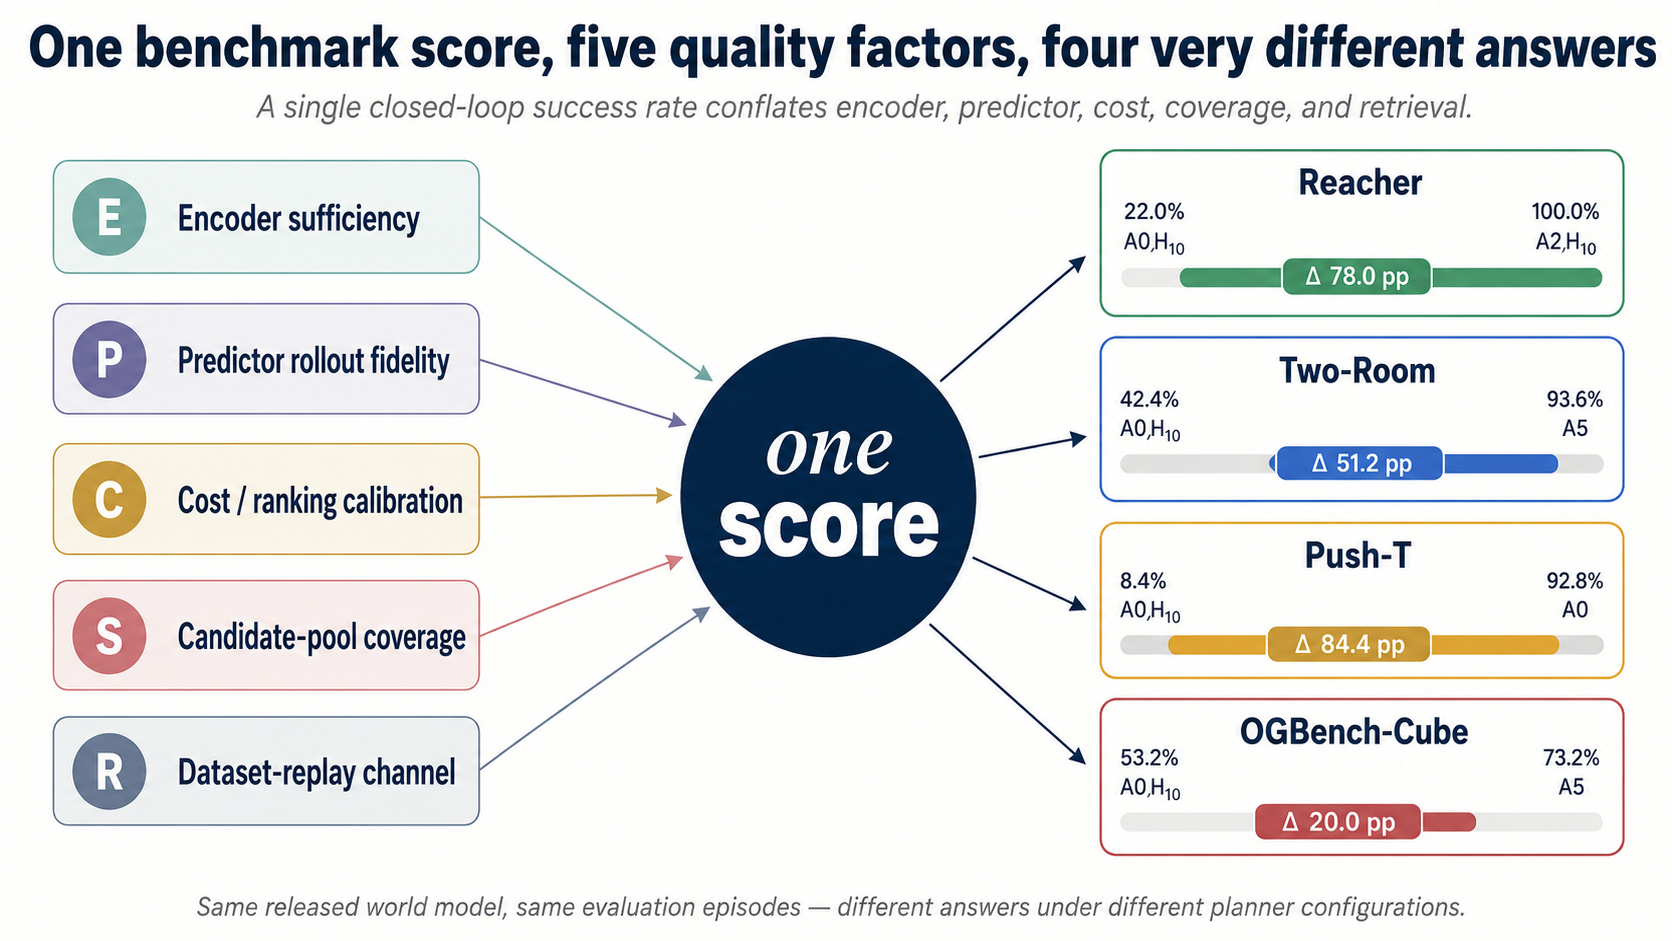
\includegraphics[width=0.78\linewidth]{fig6_composite_score_hero.png}
  \caption{The composite-score problem at a glance. Five quality factors (encoder $E$, predictor rollout $P$, cost calibration $C$, candidate coverage $S$, retrieval channel $R$) feed a single benchmark score that fans out to dramatically different per-task ranges in our 5-seed pooled grid: Reacher spans $\Delta\,78.0$ pp (A0$_{H10}$ $\to$ A2$_{H10}$), Two-Room $\Delta\,51.2$ pp, Push-T $\Delta\,84.4$ pp, OGBench-Cube $\Delta\,20.0$ pp. The same released world model is held fixed across all four; the only variation is the planner cell.}
  \label{fig:hero}
\end{figure}

\paragraph{Contributions.}
We propose a \emph{planner-calibrated evaluation protocol} that, holding the world model fixed, reports per-episode (i)~a compute frontier of vanilla iCEM, (ii)~retrieval-only leakage baselines with and without same-episode chunks, (iii)~cost-replacement controls with held-out validation, (iv)~an action-prior intervention strand, and (v)~expert-replay sanity, then assigns each episode (or task) to one of four interpretable classes: \emph{calibration-only}, \emph{coverage-bound action-prior-amenable}, \emph{coverage-bound action-prior-resistant}, or \emph{narrow-funnel / planner-frontier-resistant}. We validate the protocol on the released LeWorldModel checkpoint across all four of its evaluation tasks (Two-Room, Reacher, Push-T, OGBench-Cube), instantiating the action-prior strand as \textbf{Action-Manifold Bridge (AMB)} -- an offline-action-chunk warm start for iCEM's iter-0 elite buffer; learned policies, diffusion priors, or skill priors could be substituted in the same slot. The case study surfaces planner-axis sensitivity, a same-trajectory retrieval channel, and a cost-calibration warning for latent-WM benchmarks (replacement costs validated on encoded latents do not transfer reliably to predictor-rollout latents). We argue for per-class, planner-saturated reporting as a benchmark-design recommendation and provide a minimum-reporting-fields template.

The paper proceeds as follows. \S\ref{sec:related-work} situates the work in the literature. \S\ref{sec:protocol} defines the protocol. \S\ref{sec:sensitivity} presents protocol-sensitivity and cost / leakage diagnostics. \S\ref{sec:taxonomy} instantiates the action-prior strand and reports the four-class case-study taxonomy. \S\ref{sec:recommendation} states the benchmark-reporting recommendation and closes with limitations.

\section{Related work}
\label{sec:related-work}

\paragraph{Latent-dynamics world models.}
Model-based reinforcement learning (MBRL) with learned latent dynamics has a decade-long lineage~\cite{moerland2023mbrlsurvey,polydoros2017robotmbsurvey}: PILCO~\cite{deisenroth2011pilco}, PETS~\cite{chua2018pets}, World~Models~\cite{ha2018worldmodels}, PlaNet~\cite{hafner2019planet}, the Dreamer family~\cite{hafner2020dreamer,hafner2021dreamerv2,hafner2023dreamerv3}, MuZero~\cite{schrittwieser2020muzero}, SimPLe~\cite{kaiser2020simple}, and TD-MPC/TD-MPC2~\cite{hansen2022tdmpc,hansen2024tdmpc2}; embed-to-control~\cite{watter2015embed} and visuomotor policies~\cite{levine2016visuomotor} predate them, and value-expansion~\cite{buckman2018steve,feinberg2018mve,pong2018tdmodels}, planning-network~\cite{tamar2016vin,oh2017vpn,farquhar2018treeqn,racaniere2017iaa}, and visual-foresight~\cite{ebert2018visualforesight} variants explore adjacent design choices. Joint-embedding predictive architectures (JEPA)~\cite{assran2023ijepa,balestriero2025lejepa} and frozen visual backbones~\cite{oquab2023dinov2,nair2022r3m} have driven a wave of representation-first latent world models including DINO-WM~\cite{zhou2025dinowm}, PLDM~\cite{sobal2025pldm}, and LeWorldModel~\cite{maes2026leworldmodel}; these are trained without a reward signal and without a policy or value learner, but are deployed in the closed-loop control regime built by the MBRL lineage above.

\paragraph{Planners and trajectory generative models.}
The inference-time optimisers reused by latent-WM pipelines come from sampling-based model-predictive control (MPC) -- the Cross-Entropy Method (CEM~\cite{rubinstein2004crossentropy}), its sample-efficient variant iCEM~\cite{pinneri2020icem}, and Model Predictive Path Integral control (MPPI~\cite{williams2017mppi}) -- and from latent-space collocation~\cite{rybkin2021latco}. Trajectory generative models such as Trajectory Transformer~\cite{janner2021trajectorytransformer}, Decision Transformer~\cite{chen2021decisiontransformer}, Diffuser~\cite{janner2022diffuser}, and Diffusion Policy~\cite{chi2025diffusionpolicy} replace the inner-loop optimiser with a generative prior over actions or trajectories. Concurrent latent-WM systems including HWM~\cite{zhang2026hwm}, PiJEPA~\cite{chahe2026pijepa}, LUMOS~\cite{nematollahi2025lumos}, and Predictable Skills~\cite{guertler2025predictableskills} augment the planner side with hierarchy, language conditioning, or skill structure. Together these results show that ``world-model quality'' and ``planner-stack quality'' are separable axes; no published protocol explicitly disentangles them inside benchmark reporting, which is the gap our protocol targets.

\paragraph{Benchmarks and evaluation methodology.}
Goal-conditioned RL provides the evaluation regime we audit: UVFA~\cite{schaul2015uvfa}, HER~\cite{andrychowicz2017her}, RIG~\cite{nair2018rig}, Skew-Fit~\cite{pong2020skewfit}, UPN~\cite{srinivas2018upn}, and DBC~\cite{zhang2021dbc} establish the goal-conditioned framing. Offline / goal-conditioned RL benchmarks include D4RL~\cite{fu2020d4rl}, Meta-World~\cite{yu2020metaworld}, RLBench~\cite{james2020rlbench}, robomimic~\cite{mandlekar2021robomimic}, CALVIN~\cite{mees2022calvin}, the DeepMind Control Suite~\cite{tassa2018dmcontrol}, OGBench~\cite{park2025ogbench}, and the outward-looking WorldPrediction benchmark~\cite{chen2025worldprediction}, alongside robot-manipulation foundation models RT-1/RT-2~\cite{brohan2022rt1,brohan2023rt2}; standard background is in~\cite{sutton2018rlintro}. The evaluation-rigour literature has long flagged unstable aggregates, weak uncertainty reporting, and protocol-dependent conclusions in deep RL~\cite{henderson2018drltm,agarwal2021precipice}; we extend that lens specifically to latent-world-model benchmarks.

\paragraph{Action-prior interventions.}
A separate strand of work asks whether a learned or retrieval-based prior over actions can move the closed-loop number even when the world model is held fixed. Diffusion Policy~\cite{chi2025diffusionpolicy} and Diffuser~\cite{janner2022diffuser} treat the action prior as a generative model; Trajectory Transformer~\cite{janner2021trajectorytransformer} and Decision Transformer~\cite{chen2021decisiontransformer} treat it as autoregressive sequence prediction; LUMOS~\cite{nematollahi2025lumos} couples a language-conditioned prior to a world-model planner; Predictable Skills~\cite{guertler2025predictableskills} compose skill-level priors into long-horizon plans. Our protocol exposes this design space as a methodology-agnostic ``action-prior hook'': any admissible mechanism for biasing or initialising the planner's candidate distribution under benchmark-defined leakage exclusions can be slotted in. We instantiate the hook with Action-Manifold Bridge (AMB), an offline-action-chunk warm start for iCEM, but the slot itself is the primary construct.

\paragraph{Where this paper sits.}
Most of the literature above is method-side: it proposes a better world model, a better planner, or a better benchmark. Our contribution is orthogonal. We hold the released world model fixed and audit how planner schedule, cost, action prior, and retrieval channel jointly determine the closed-loop number that current latent-WM benchmarks report. The protocol below borrows the closed-loop control regime from the MBRL lineage and the inference-time optimisers from sampling-based MPC, but adds a per-episode failure-class taxonomy that lets a reader attribute differences across world models or planner versions to specific components rather than to a single conflated aggregate. In this sense the protocol complements rather than competes with the works above: any of the latent-WM systems referenced here could be plugged into the same harness and reported under the same per-class scheme. The closest precedents are the deep-RL evaluation-rigour critiques~\cite{henderson2018drltm,agarwal2021precipice} and benchmark-design papers such as OGBench~\cite{park2025ogbench}, which argue for capability-targeted reporting; we extend that stance into the latent-world-model regime where the benchmark score is composed not only of model quality but of an entire planner stack.

\section{Planner-calibrated diagnostic protocol}
\label{sec:protocol}

\begin{figure}[t]
  \centering
  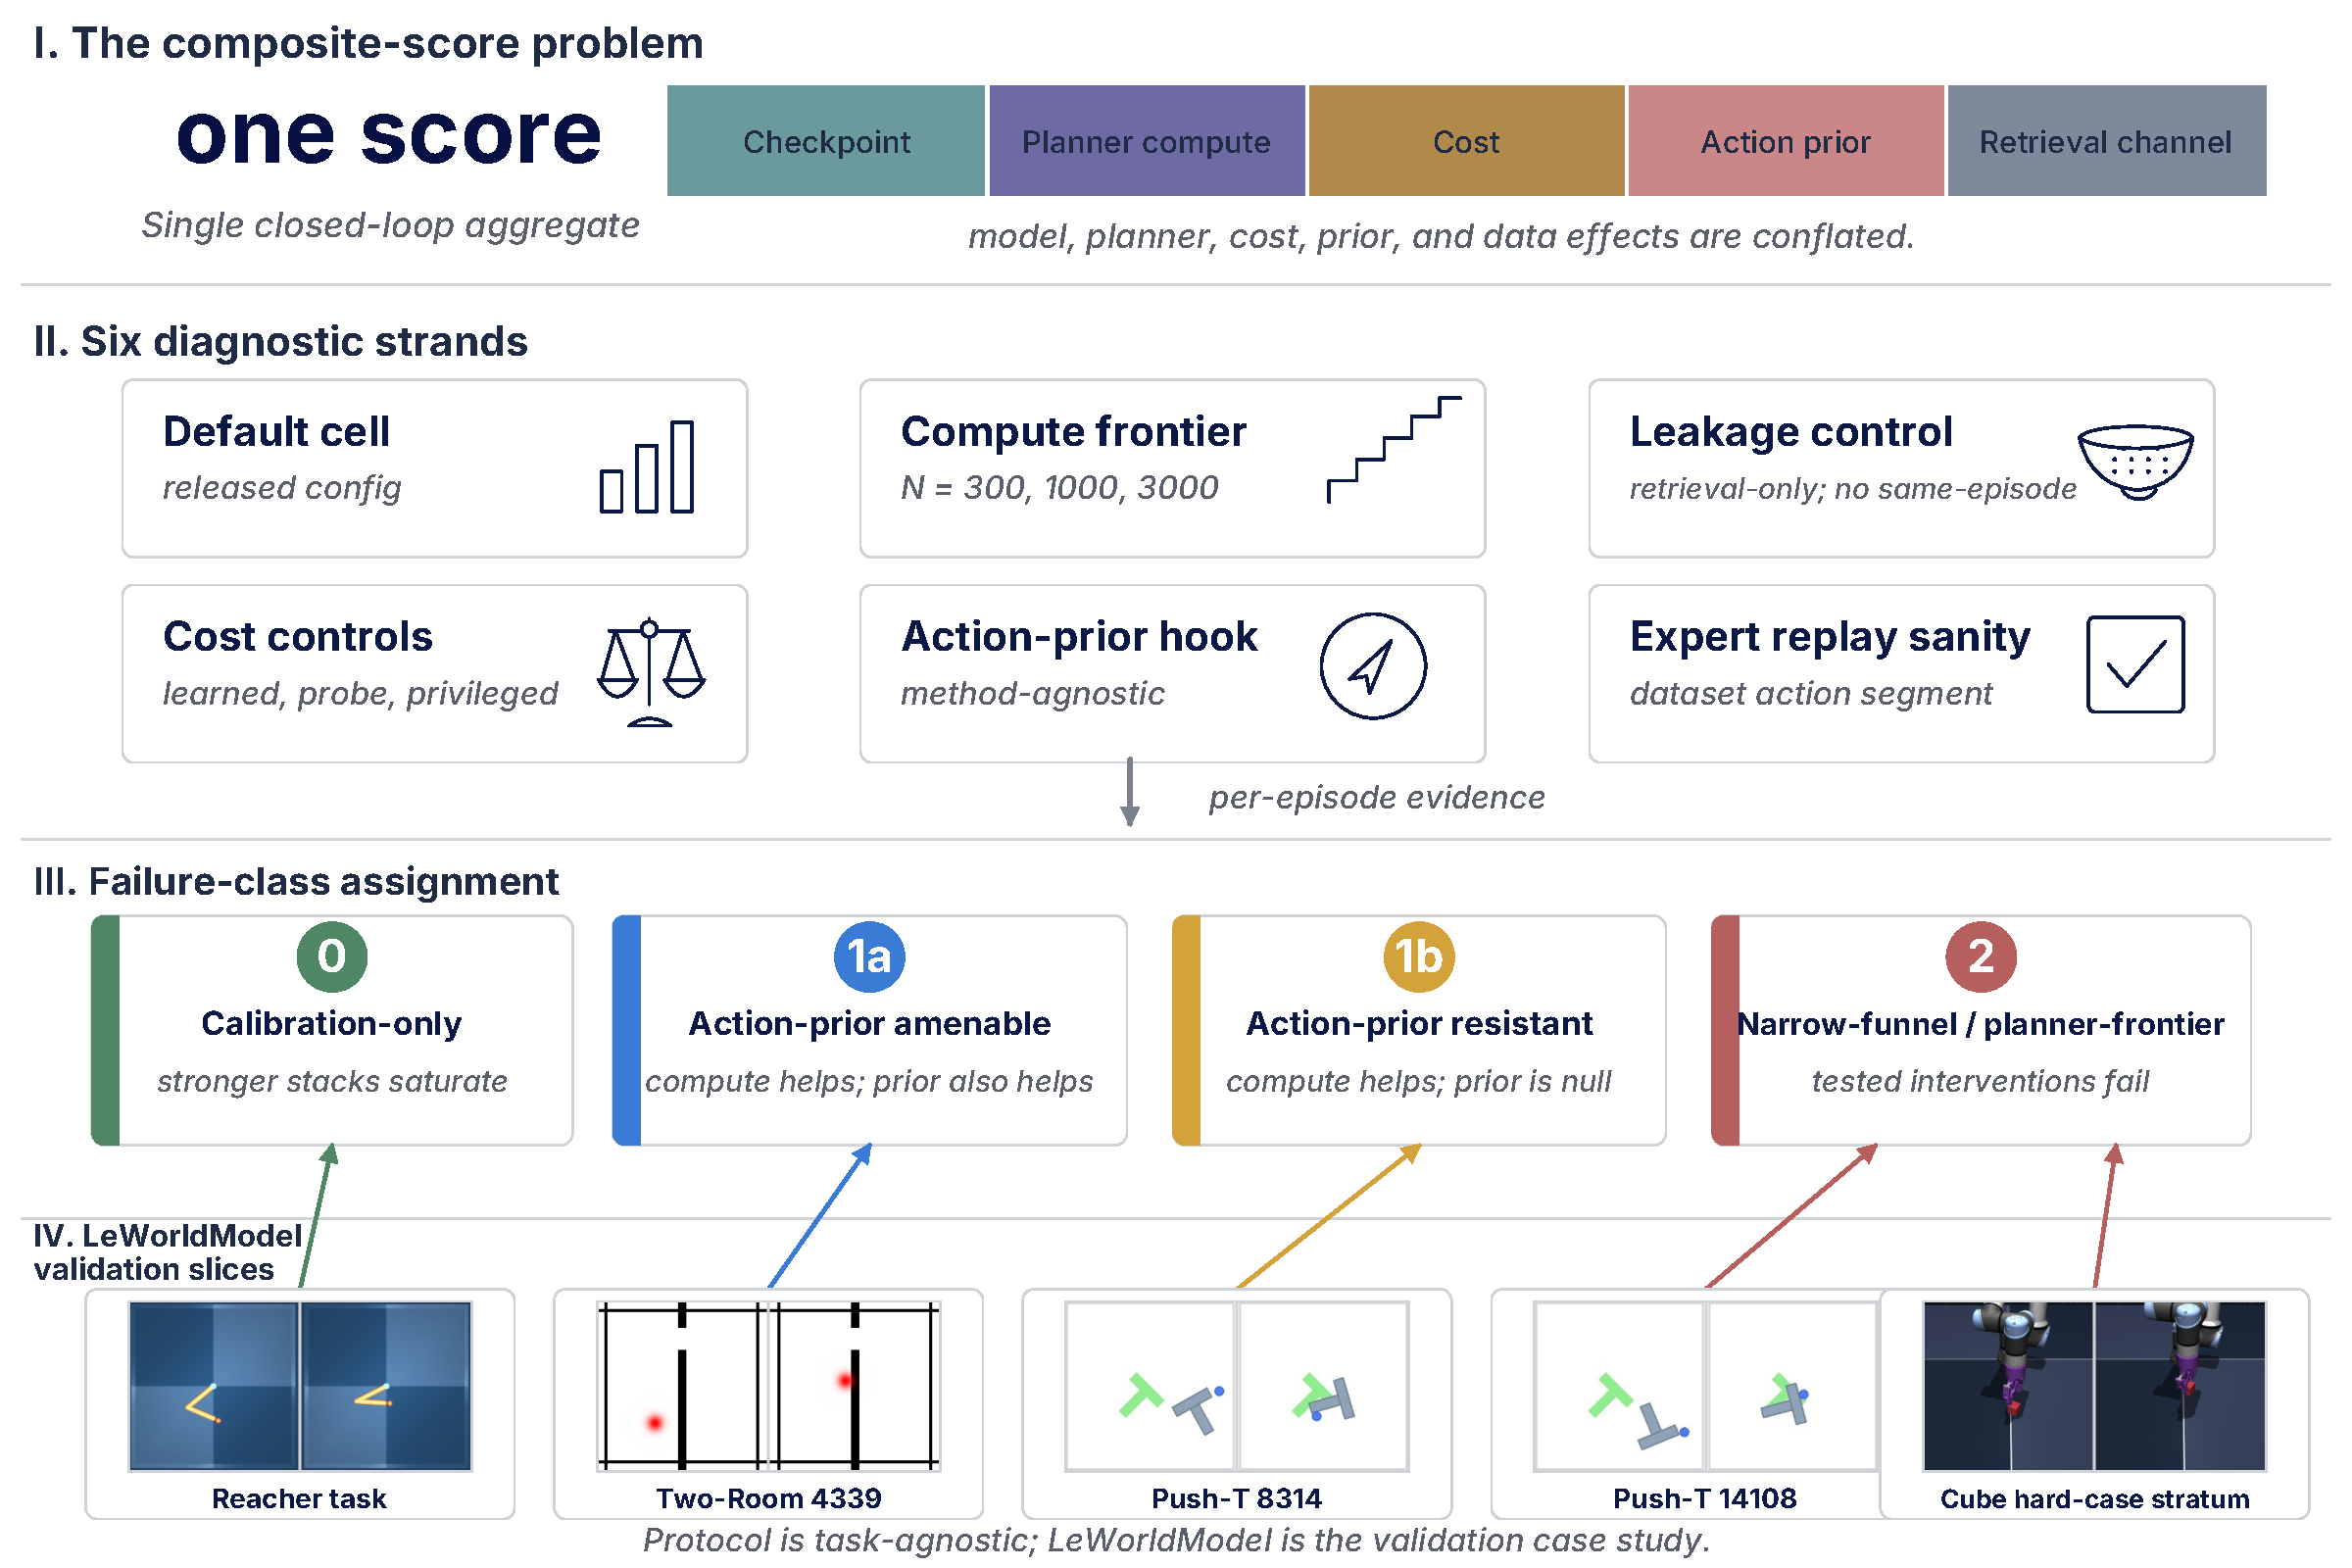
\includegraphics[width=0.85\linewidth]{fig1_planner_calibrated_diagnostics_overview.pdf}
  \caption{Per-episode planner-calibrated evaluation protocol. Six diagnostic strands (published-style A0, compute frontier, retrieval-only leakage, cost-replacement, action-prior hook, expert replay sanity) feed a per-episode failure-class assignment over four classes (0 calibration-only, 1a action-prior-amenable, 1b action-prior-resistant, 2 narrow-funnel / planner-frontier-resistant); the per-task report aggregates per class. The action-prior hook is a method-agnostic slot; AMB-random / AMB-topK populate it in this study.}
  \label{fig:protocol}
\end{figure}

\paragraph{Setup and notation.}
Each evaluation episode is a tuple $(\text{world model}, \text{episode index}, \text{start step}, \text{goal step})$ drawn by the benchmark's eval-set sampler; we hold the world model and dataset fixed and vary only the planner stack. The planner is sampling-based model-predictive control (MPC): at each control step it draws $N$ candidate action sequences of length $H$ (the \emph{planning horizon}), scores each under the latent world model, and executes the first $RH$ actions of the lowest-cost candidate before re-planning ($RH$ is the \emph{receding-horizon stride}, both in environment steps). We use the Cross-Entropy Method (CEM~\cite{rubinstein2004crossentropy}) and its sample-efficient variant iCEM~\cite{pinneri2020icem}; \emph{warm-start} seeds the next plan with the previous plan's top-scoring (``elite'') candidates. The default cost is the latent $L_2$ distance from the predicted latent $z_t$ to the goal latent $z_g$ at the final predicted step (\emph{terminal}) or summed over the rollout (\emph{cumulative}). The benchmark fixes per-task evaluation episodes $\mathit{num\_eval}=50$ and runs each in its own environment process ($\mathit{solver\_batch\_size}=1$). Success rates are reported in percentage points (pp) with Wilson $95\%$ binomial confidence intervals; paired comparisons use the paired bootstrap and McNemar's exact test on shared (episode, seed) pairs. We use the released LeWorldModel checkpoint~\cite{maes2026leworldmodel} across its four evaluation tasks (Two-Room, Reacher, Push-T, OGBench-Cube); nothing in the protocol is specific to it.

\paragraph{Diagnostic strands.}
For each episode we report the following six strands. Each strand is a small set of planner ``cells'' -- specific configurations of $(\text{solver}, H, RH, \text{cost}, \text{warm-start}, N)$ -- run paired on the same episode-seed grid as the others. The notation $A_0, A_1, \dots, A_5$ labels six stacked configurations introduced in \S\ref{subsec:perturb-grid} below; $A_{0,H10}$ and $A_{2,H10}$ are horizon-isolation variants at $H{=}10$.

\begin{description}[itemsep=2pt,topsep=2pt,leftmargin=2em]
\item[Published-style cell ($A_0$).] CEM with $H{=}5$, $RH{=}5$, terminal latent-distance cost, no warm-start, at the published candidate-sample budget $N{=}300$. Reproduces the default LeWM eval.
\item[Compute frontier ($A_5$).] iCEM with $H{=}10$, $RH{=}1$, cumulative latent-distance cost, warm-start, at three sample budgets $N \in \{300, 1000, 3000\}$. Tests whether the headline number is planner-budget limited.
\item[Cost-replacement controls.] The latent $L_2$ cost is swapped for a learned or probe-decoded alternative (validated on held-out episodes) and scored on predictor-rollout latents at $N{=}300$ inside the $A_5$ stack. Tests whether the cost is the binding constraint.
\item[Action-prior hook.] Any admissible mechanism that biases or initialises the planner's candidate action distribution under the benchmark's leakage exclusions (\S\ref{sec:taxonomy}). Tests whether a stronger prior over actions closes the gap.
\item[Retrieval-only leakage baseline.] The top $K{=}10$ offline action chunks (ranked by latent-endpoint nearest-neighbour to the eval $(z_t, z_g)$) are executed open-loop in the simulator, reported separately with and without same-episode chunks. The same-episode variant is a leakage diagnostic, not a model score.
\item[Expert replay.] Replay the dataset action segment for the $(\text{start}, \text{goal})$ pair as a sanity check that the evaluation pair admits a dataset-supported solution at all.
\end{description}

Table~\ref{tab:protocol-card} summarizes the strands as a reusable protocol card: diagnostic question, required benchmark inputs, output to report, and how each strand is instantiated in our controlled validation case study. The card is the artifact a benchmark author would implement; the instantiation column documents only the LeWorldModel-specific cells used here.

\begin{table}[ht]
\centering\footnotesize
\caption{Planner-calibrated protocol card for latent world-model benchmark reports. Strand definitions and the reporting interface are task-agnostic; the rightmost column documents how each strand is instantiated in our controlled validation case study on the released LeWorldModel checkpoint.}
\label{tab:protocol-card}
\renewcommand{\arraystretch}{1.05}
\begin{tabularx}{\textwidth}{@{}>{\raggedright\arraybackslash}p{2.0cm}>{\raggedright\arraybackslash}X>{\raggedright\arraybackslash}X>{\raggedright\arraybackslash}p{2.5cm}>{\raggedright\arraybackslash}p{3.1cm}@{}}
\toprule
Strand & Diagnostic question & Required benchmark inputs & Output to report & Instantiation here \\
\midrule
Published-style cell & What score does the default planner give? & Released checkpoint; eval-set sampler; default planner config & Default closed-loop success; exact planner settings & A0 (CEM, $H{=}5$, $RH{=}5$, terminal cost, $N{=}300$) \\
Compute frontier & Is the score planner-budget limited? & Same episodes; paired planner seeds; increasing candidate budgets / horizons & Per-episode and per-task success over tested budgets; planner gap & vanilla iCEM at $N \in \{300, 1000, 3000\}$ \\
Retrieval-only leakage & Can dataset retrieval solve without model rollout? & Offline action chunks; same-ep inclusion / exclusion flag & Same-ep and no-same-ep retrieval-only success & Best-of-$K{=}10$ open-loop chunks \\
Cost-replacement controls & Is terminal latent distance the limiting cost? & Held-out cost validation; predictor-rollout scoring & Learned / probe / privileged-cost cell success; validation metric & Q-cost, probe-xy, contact-cost cells \\
Action-prior hook & Does a structured action prior or candidate bias close coverage-bound cases? & Any admissible action-prior or candidate-generation mechanism; leakage exclusions & Paired delta vs.\ default at matched budget & AMB-random / AMB-topK at $N{=}300$, no-same-ep \\
Expert replay sanity & Is the episode physically solvable under dataset actions? & Dataset action segment or equivalent oracle & Replay success / failure & Scripted expert replay in simulator \\
\bottomrule
\end{tabularx}
\end{table}

\paragraph{Failure-class assignment.}
From the strands above, each episode or task slice is classified into one of four classes (\emph{0.~calibration-only}, \emph{1a.~coverage-bound, action-prior-amenable}, \emph{1b.~coverage-bound, action-prior-resistant}, or \emph{2.~narrow-funnel / planner-frontier-resistant}); class definitions and diagnostic signatures are in Figure~\ref{fig:taxonomy-showcase}. ``Dominates'' requires a paired-bootstrap $95\%$ CI on the mean delta excluding zero and a one-sided discordant pattern in the McNemar table; ``improves strongly'' allows small reverse-direction discordant counts (\S\ref{sec:taxonomy}). The protocol is task-agnostic in what it holds fixed and varies: a world-model checkpoint, eval-set sampler, planner compute, candidate proposal distribution, cost function, retrieval channel, and replay sanity. Our empirical validation is narrower (one released LeWorldModel checkpoint family, four tasks), so we claim portability of the diagnostic design, not universality of the observed class mix or of AMB's effectiveness.

\section{Protocol sensitivity and diagnostic controls}
\label{sec:sensitivity}

\subsection{Single-axis planner perturbations can drop success by 84 points}
\label{subsec:perturb-grid}

We perturb the published planner along five axes, holding the world model fixed: solver (CEM $\to$ iCEM~\cite{pinneri2020icem}), $RH \in \{5, 1\}$, cost shape (terminal $\to$ cumulative latent distance), warm-start (off $\to$ on), and $H \in \{5, 10\}$. Each subsequent cell $A_1,\dots,A_5$ keeps every prior change and applies one additional axis; $A_{0,H10}$ and $A_{2,H10}$ isolate the horizon change at $RH{=}5$ and $RH{=}1$. Figure~\ref{fig:perturb-heatmap} summarises the four-task grid; all four task rows are pooled over five Hydra-coupled seeds $\{0,1,2,3,42\}$ for $n=250$ trials per cell (exact values in appendix Table~\ref{tab:perturb}). The ``best'' cell is task-specific: cumulative cost (A2 onwards) saturates Reacher above $99\%$, helps Two-Room and Cube modestly, and partially recovers Push-T after a sharp $RH{=}1$ collapse. \emph{No single perturbation helps every task}, so any single planner choice is at best a compromise. The most striking single-axis effects are on Push-T: $A_0 \to A_1$ ($RH{=}5{\to}1$) drops from $92.8\%$ to $22.0\%$ and $A_0 \to A_{0,H10}$ ($H{=}5{\to}10$) drops to $8.4\%$ -- swings of $70.8$ and $84.4$\,pp respectively (dark outline in Figure~\ref{fig:perturb-heatmap}; mechanism in Appendix~\ref{app:sensitivity-summary}).

\begin{figure}[ht]
  \centering
  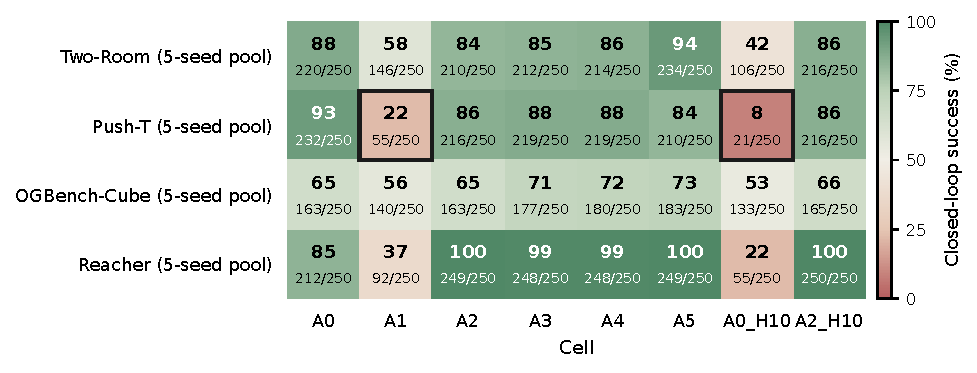
\includegraphics[width=0.96\linewidth]{fig2_four_task_sensitivity_heatmap.pdf}
  \caption{Four-task planner-perturbation grid (closed-loop success \%; $k/n$ shown below each cell, all $n=250$). All four task rows pool five Hydra-coupled seed runs $\{0,1,2,3,42\}$ ($50$ episodes per seed, cells paired within seed). Columns: A0..A5 stacked single-axis perturbations and the horizon-isolation cells A0$_{H10}$, A2$_{H10}$. Dark outlines mark the largest single-axis collapses on Push-T (A0$\to$A1: $-70.8$\,pp; A0$\to$A0$_{H10}$: $-84.4$\,pp). Exact values in Table~\ref{tab:perturb}; per-seed breakdowns in \texttt{grid-path2-summary.json} (Reacher per-seed in Table~\ref{tab:reacher-5seed} for App.~\ref{app:reacher}).}
  \label{fig:perturb-heatmap}
\end{figure}

\subsection{Seed sensitivity at the published budget}
\label{subsec:seed-fragility}

Under the released LeWM Two-Room evaluation, which batches $16$ episodes per environment process, the $A_5$ cell scores $100\%$ on the single hardest episode (eval index 4, episode 4339). When we re-run 4339 in isolation -- one episode, one environment, $100$ independent CEM seeds -- success drops to $63/100 = 63\%$ (Wilson $95\%$ CI $[53, 72]$) at the published candidate budget $N{=}300$, and rises to $100/100$ ($[96, 100]$) at $N{=}1000$. The headline $100\%$ in the batched arrangement was therefore contingent on the specific sample stream drawn for that environment slot, not on a stable property of the world model. Closed-loop success on Two-Room and Push-T depends on planner configuration, CEM sample stream, and how episodes are batched at evaluation time.

\subsection{Cost replacement strictly hurts (predictor distribution shift)}
\label{subsec:cost-replace}

We swap the latent-distance cost inside the $A_5$ stack with two alternatives. \textbf{Q v2-cost} is a learned reachability classifier (validation AUC $0.78$); \textbf{probe-xy cost} is a Ridge probe decoding agent position from the latent (train pixel error $3.85$\,px). Both give $0/10$ on TwoRoom~4339, strictly worse than the $5/10$ matched-$n$ vanilla baseline. A privileged pusher--block contact cost gives $0/5$ on both PushT 8314 and PushT 14108 (strictly worse than the $1/5$ vanilla baselines). Full results in Appendix~\ref{app:cost-replacement} (Table~\ref{tab:cost}). The Q v2 classifier itself is \emph{not} broken: on encoded true latents it ranks the failed-$A_5$ trajectory at $0.04$ probability of reach and a frame $200$ steps beyond the horizon at $0.000$. The failure is at the interface: the planner scores predictor-rollout latents, which lie on a slightly different distribution than the encoded latents Q v2 was trained on. \emph{Cost-calibration warning}: learned costs should be reported with both an encoded-latent validation metric \emph{and} a predictor-rollout closed-loop number.

\subsection{Same-trajectory goal sampling opens a $30$-point retrieval channel}
\label{subsec:leakage}

The published evaluation samples (start,~goal) frames from the same training trajectory, which puts a near-solution action sequence in the dataset itself. We test how much of the published score is attributable to retrieval rather than world-model rollout. For TwoRoom~4339, we retrieve the top-$K{=}10$ latent-endpoint-nearest offline action chunks and execute each open-loop in the simulator (no iCEM, no world-model rollout). With same-episode chunks allowed, $8/10 = 80\%$ of trials succeed; with same-episode chunks excluded, $5/10 = 50\%$ -- a $30$-percentage-point difference that current LeWM evaluations do not report. On PushT~14108 the same retrieval-only baseline is $0/10$, a useful control showing the leakage is task-geometry-dependent. Figure~\ref{fig:retrieval-leakage} (Appendix~\ref{app:retrieval-leakage-fig}) plots the paired bars.

\section{Action-prior strand and failure taxonomy}
\label{sec:taxonomy}

\subsection{One action-prior instantiation: Action-Manifold Bridge (AMB)}

AMB augments iCEM with an offline-action-chunk warm-start. We pre-compute, from the offline dataset, a database of length-$H$ \emph{action chunks}: each chunk $c$ is a contiguous sequence of $H$ training actions, tagged with its first- and last-frame latents $z_c^{\text{start}}$ and $z_c^{\text{end}}$. At plan time, given $(z_t, z_g)$, AMB-topK retrieves the top-$K$ chunks by $\text{score}(c) = \|z_t - z_c^{\text{start}}\|^2 + \|z_g - z_c^{\text{end}}\|^2$, injects them as the iteration-0 elite buffer of iCEM, and lets iCEM continue as usual. \textbf{AMB-random} replaces the nearest-neighbour ranking with uniform sampling as a mechanism ablation. For benchmark integrity we exclude the evaluation episode from the retrieval database (\emph{no-same-episode retrieval}). Endpoint-NN retrieval selects chunks whose probe-decoded start/end positions are $2$--$3\times$ closer to the eval $(\text{start}, \text{goal})$ than random chunks (Appendix~\ref{app:retrieval-quality}).

\paragraph{Other action-prior instantiations.}
AMB is one way to populate the action-prior hook. Alternatives include learned policy warm-starts (Decision Transformer~\cite{chen2021decisiontransformer}, Trajectory Transformer~\cite{janner2021trajectorytransformer}), diffusion action priors~\cite{chi2025diffusionpolicy,janner2022diffuser}, language-conditioned warm-starts~\cite{nematollahi2025lumos,chahe2026pijepa}, and skill priors~\cite{guertler2025predictableskills}. Broader planner-side alternatives such as value-guided MPC~\cite{hansen2024tdmpc2} or latent-space collocation~\cite{rybkin2021latco} test adjacent protocol dimensions. We do not evaluate substitutes here; admissible alternatives should be reported under the same leakage exclusions and paired fixed-budget comparisons.

\subsection{TwoRoom~4339: AMB closes the seed-fragile gap}

On the $100$-seed paired sweep, AMB-topK no-same-episode reaches $85/100$ ($[77, 91]$), a paired $+22$\,pp improvement over vanilla $A_5$ at $N{=}300$. Table~\ref{tab:paired-stats} summarises paired-difference statistics for TwoRoom~4339 and the two Push-T hard episodes. Each paired (seed, episode) outcome is concordant (both methods succeed, or both fail) or discordant (one succeeds, the other fails); the McNemar test asks whether the two discordant directions are imbalanced. On TwoRoom~4339 the ``baseline succeeds but intervention fails'' count is exactly zero for every comparison: every vanilla success is also an AMB-topK success, and every AMB-topK success is also an $N{=}1000$ success (strict dominance). AMB and $N{=}1000$ trade off: AMB is $\sim 2.2\times$ cheaper in wall-clock and $\sim 3.3\times$ cheaper in model queries but has a residual $\sim 15\%$ failure rate, while $N{=}1000$ saturates. The full TwoRoom~4339 forest plot is in Appendix~\ref{app:tworoom-mechanism-fig}.

\subsection{Cross-task transfer: AMB does not help Push-T}

We extend three cells per Push-T hard episode (vanilla $N{=}300$, vanilla $N{=}1000$, AMB-topK no-same-ep) plus AMB-random no-same-ep on PushT~8314 to $20$ paired CEM seeds.

\begin{table}[ht]
\centering\footnotesize
\caption{Paired-difference statistics (paired bootstrap $B{=}20{,}000$; McNemar exact two-sided $p$). TwoRoom~4339 uses 100 paired CEM seeds; PushT 8314 / 14108 use 20 paired seeds. On TwoRoom~4339 every B$>$A discordant count is zero (strict dominance).}
\label{tab:paired-stats}
\renewcommand{\arraystretch}{1.05}
\begin{tabularx}{\textwidth}{@{}>{\raggedright\arraybackslash}p{2.4cm}>{\raggedright\arraybackslash}X r r r@{}}
\toprule
Slice & Comparison & $\Delta$ (pp) & 95\% CI & Discordant pairs; $p$ \\
\midrule
\multicolumn{5}{@{}l}{\textit{TwoRoom 4339 ($n{=}100$)}} \\
& AMB-topK $-$ vanilla $N{=}300$        & $\mathbf{+22}$ & $[+14, +30]$ & $22/0$; $\mathbf{4.8\times10^{-7}}$ \\
& vanilla $N{=}1000 - N{=}300$          & $\mathbf{+37}$ & $[+28, +47]$ & $37/0$; $\mathbf{1.5\times10^{-11}}$ \\
& vanilla $N{=}1000 -$ AMB-topK         & $\mathbf{+15}$ & $[+8, +22]$  & $15/0$; $\mathbf{6.1\times10^{-5}}$ \\
\midrule
\multicolumn{5}{@{}l}{\textit{PushT 8314 ($n{=}20$)}} \\
& AMB-topK $-$ vanilla $N{=}300$        & $+0$           & $[-25, +25]$ & $3/3$; $1.0$ \\
& AMB-random $-$ vanilla $N{=}300$      & $+5$           & $[-15, +25]$ & $3/2$; $1.0$ \\
& vanilla $N{=}1000 - N{=}300$          & $\mathbf{+60}$ & $[+40, +80]$ & $12/0$; $\mathbf{4.9\times10^{-4}}$ \\
\midrule
\multicolumn{5}{@{}l}{\textit{PushT 14108 ($n{=}20$)}} \\
& AMB-topK $-$ vanilla $N{=}300$        & $-5$           & $[-20, +10]$ & $1/2$; $1.0$ \\
& vanilla $N{=}1000 - N{=}300$          & $+0$           & $[-20, +20]$ & $2/2$; $1.0$ \\
\bottomrule
\end{tabularx}
\end{table}

\textbf{PushT 8314 is coverage-bound but action-prior-resistant.} $N{=}1000$ improves strongly over $N{=}300$ ($+60$\,pp, $p = 4.9\times10^{-4}$), but neither AMB-topK nor AMB-random improves at the published budget (both $\Delta \approx 0$, $p = 1.0$). \emph{The effectiveness of this AMB instantiation is task-class-specific; the action-prior strand is diagnostic rather than assumed beneficial.}

\textbf{PushT 14108 is narrow-funnel and planner-frontier-resistant.} $N{=}1000$ does not improve over $N{=}300$ ($\Delta = 0$, $p = 1.0$); AMB does not help; a privileged probe-decoded contact cost (latent~$L_2 + \lambda \cdot \text{pusher--block distance}$) gives $0/5$. Per-step traces show the pusher rarely approaches the block within the 10-step planning horizon. Expert replay succeeds, but no tested intervention reliably improves over the low $\sim 10\%$ vanilla baseline. Figure~\ref{fig:pusht-hardcases} compares all four primitives.

\begin{figure}[ht]
  \centering
  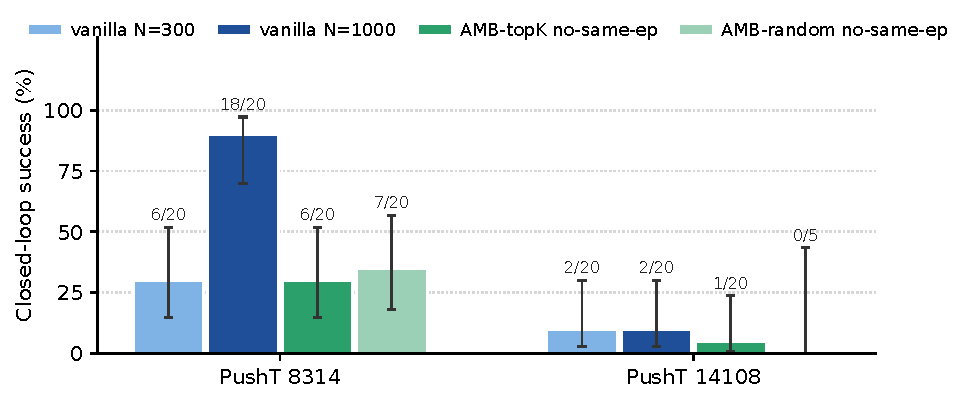
\includegraphics[width=0.92\linewidth]{fig3c_pusht_hardcases.pdf}
  \caption{PushT hard cases (grouped bars; Wilson 95\% CI whiskers; $k/n$ above bars). On PushT~8314 only the $N{=}1000$ compute-frontier cell improves over vanilla ($18/20$ vs.\ $6/20$); both AMB variants stay near the vanilla rate, anchoring class~1b. On PushT~14108 no tested cell reliably improves over the low $\sim 10\%$ vanilla baseline, anchoring class~2.}
  \label{fig:pusht-hardcases}
\end{figure}

\subsection{Four-class failure taxonomy across the four LeWM tasks}

Combining the AMB results with the four-task perturbation grid (\S\ref{subsec:perturb-grid}) and the Cube hard-case sweep (Appendix~\ref{app:cube-hardcase}), we adopt the four-class taxonomy summarised in Figure~\ref{fig:taxonomy-showcase}. Class labels are generic over the action-prior strand: any other intervention (a learned policy, a diffusion prior, AMB) would inherit the same structure with the primitive substituted in the diagnostic signature.

\begin{figure}[ht]
  \centering
  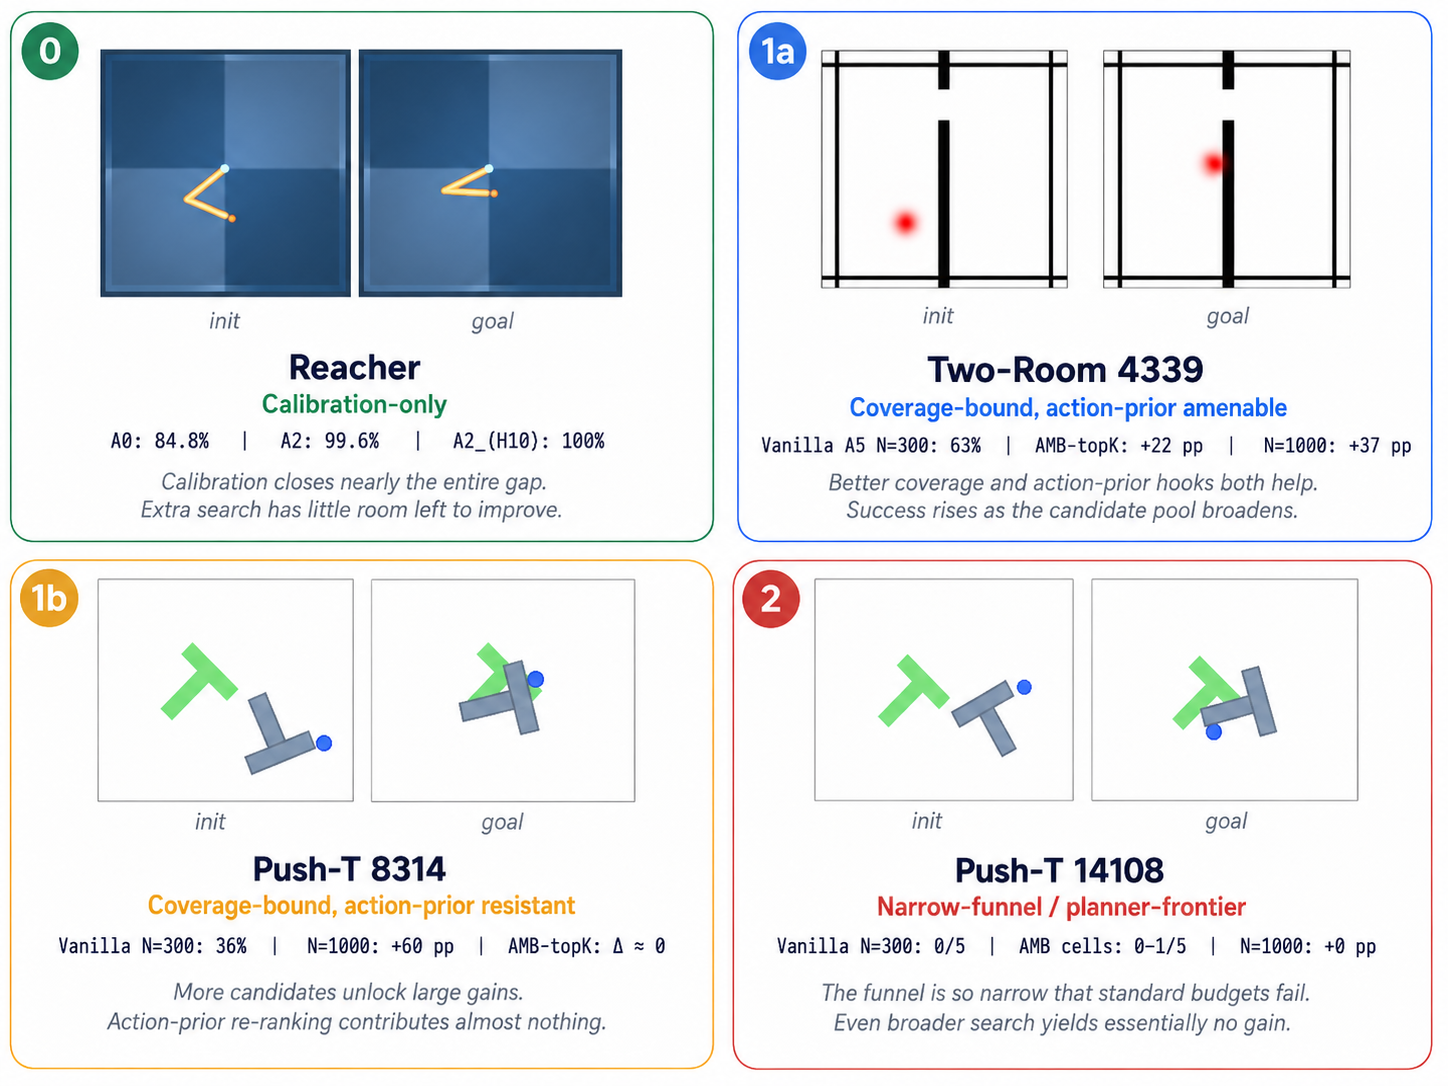
\includegraphics[width=0.72\linewidth]{fig5_taxonomy_showcase.png}
  \caption{Four-class taxonomy showcase. Each panel pairs a real init / goal frame composite with the cell signature that anchors the class assignment. \textbf{Class~0} (sage) saturates on Reacher; \textbf{1a} (slate) closes on TwoRoom~4339 under either stronger compute or the AMB-topK action-prior; \textbf{1b} (amber) yields to compute alone on PushT~8314 but remains null under AMB; \textbf{2} (rose) is the planner-frontier-resistant stratum where PushT~14108 and the Cube hard-case episodes register $\le\!22\%$ across every tested cell. Class colours match Band~III of Figure~\ref{fig:protocol} and the dark-outline highlights in Figure~\ref{fig:perturb-heatmap}. Cube has a verified class-2 hard stratum (three episodes at $0/60$ across cells $\{A_0, A_4, A_5, A_{2,H10}\}$ and five solver seeds; seven $0/8$ failures in the perturbation grid) plus an easy/medium population not separately classified.}
  \label{fig:taxonomy-showcase}
\end{figure}

\textbf{Reacher} anchors class 0: cumulative-cost alone ($A_1 \to A_2$) lifts the mean from $36.8\%$ to $99.6\%$, leaving no head-room. \textbf{Cube} has an easy/medium population often solved by stronger cells (best task-level cell $A_5 = 73.2\%$ in the five-seed pool) plus a verified planner-frontier-resistant hard stratum: seven Cube episodes are $0/8$ across all eight grid cells, and a focused paired sweep on three representative failures across cells $\{A_0, A_4, A_5, A_{2,H10}\}$ and seeds $\{1,\dots,5\}$ gives $0/60$ successes. We label these cases ``planner-frontier-resistant under the tested published-budget stack,'' not ``action-prior-resistant'' (the latter would require a Cube-specific action-prior, which we did not implement). Per-primitive matrices for the three anchor slices are tabulated in Appendix~\ref{app:slice-matrices}.

\section{Benchmark recommendation}
\label{sec:recommendation}

\paragraph{Per-class, planner-saturated reporting.}
The headline benchmark number must be reported per failure class as well as per task: a single aggregate hides that no single planner primitive helps every class. Concretely, report each protocol-card cell separately (default; compute-frontier; registered action-prior hook with leakage exclusions; retrieval-only no-same-ep; cost-replacement where applicable), plus an oracle \emph{Planner Gap} = (max over primitives) $-$ default-planner score on the same episodes. Same-trajectory goal sampling must be flagged: the retrieval-only no-same-ep baseline is the per-episode hardness floor for retrieval-style methods and must be reported alongside the default score; a same-ep variant is a separate diagnostic and never combined with the headline. A slice is \emph{calibration-only} if (a) the published-planner score is at or near the per-class compute-frontier ceiling, or (b) the retrieval-only no-same-episode baseline solves a non-trivial fraction ($\geq 30\%$ in our use; the cutoff should be pre-registered per release).

\paragraph{Minimum reporting fields.}
A planner-calibrated latent-WM benchmark claim should populate seven method-agnostic fields: \textbf{default score}; \textbf{planner frontier} (gap = best $-$ default); \textbf{leakage floor} (no-same-ep retrieval-only); \textbf{cost controls} (encoded-latent validation \emph{and} predictor-rollout result); \textbf{action-prior cell} (method, admissibility, paired delta at matched budget); \textbf{failure-class mix}; and \textbf{source manifest} ($k/n$, Wilson CIs, JSON paths). The schema follows offline / goal-conditioned-RL benchmark conventions~\cite{fu2020d4rl,park2025ogbench} and deep-RL evaluation rigour~\cite{henderson2018drltm,agarwal2021precipice}; substituting another action-prior does not change it.

\paragraph{Limitations and discussion.}
\label{sec:discussion}
We do not claim LeWM's world model is bad -- only that the published-protocol score is composite -- and AMB is one example action-prior, null on PushT 1b/2 and untested on Reacher/Cube. PushT~14108 and the Cube hard stratum are unimproved by tested planner primitives, but untested alternatives (skill priors, collocation, value-guided MPC~\cite{zhang2026hwm,chahe2026pijepa}) remain open. The protocol generalises to other frozen checkpoints by reusing the protocol card.

% --- References ---
\begin{thebibliography}{99}

\bibitem{agarwal2021precipice}
R.~Agarwal, M.~Schwarzer, P.~S.~Castro, A.~Courville, M.~G.~Bellemare.
\emph{Deep Reinforcement Learning at the Edge of the Statistical Precipice.}
NeurIPS 2021 (Outstanding Paper).

\bibitem{andrychowicz2017her}
M.~Andrychowicz, F.~Wolski, A.~Ray, J.~Schneider, R.~Fong, P.~Welinder, B.~McGrew, J.~Tobin, P.~Abbeel, W.~Zaremba.
\emph{Hindsight Experience Replay.}
NeurIPS 2017.

\bibitem{assran2023ijepa}
M.~Assran, Q.~Duval, I.~Misra, P.~Bojanowski, P.~Vincent, M.~Rabbat, Y.~LeCun, N.~Ballas.
\emph{Self-Supervised Learning from Images with a Joint-Embedding Predictive Architecture.}
CVPR 2023. doi:10.1109/CVPR52729.2023.01499.

\bibitem{balestriero2025lejepa}
R.~Balestriero, Y.~LeCun.
\emph{LeJEPA: Provable and Scalable Self-Supervised Learning Without the Heuristics.}
arXiv:2511.08544, 2025.

\bibitem{brohan2022rt1}
A.~Brohan, N.~Brown, J.~Carbajal, et al.
\emph{RT-1: Robotics Transformer for Real-World Control at Scale.}
arXiv:2212.06817, 2022.

\bibitem{brohan2023rt2}
A.~Brohan, Y.~Chebotar, C.~Finn, et al.
\emph{RT-2: Vision-Language-Action Models Transfer Web Knowledge to Robotic Control.}
arXiv:2307.15818, 2023.

\bibitem{buckman2018steve}
J.~Buckman, D.~Hafner, G.~Tucker, E.~Brevdo, H.~Lee.
\emph{Sample-Efficient Reinforcement Learning with Stochastic Ensemble Value Expansion.}
NeurIPS 2018. arXiv:1807.01675.

\bibitem{chahe2026pijepa}
A.~Chahe, L.~Zhou.
\emph{Policy-Guided World Model Planning for Language-Conditioned Visual Navigation.}
arXiv:2603.25981, 2026.

\bibitem{chen2021decisiontransformer}
L.~Chen, K.~Lu, A.~Rajeswaran, K.~Lee, A.~Grover, M.~Laskin, P.~Abbeel, A.~Srinivas, I.~Mordatch.
\emph{Decision Transformer: Reinforcement Learning via Sequence Modeling.}
NeurIPS 2021.

\bibitem{chen2025worldprediction}
D.~Chen, W.~Chung, Y.~Bang, Z.~Ji, P.~Fung.
\emph{WorldPrediction: A Benchmark for High-level World Modeling and Long-horizon Procedural Planning.}
ICML 2025 World Models Workshop.

\bibitem{chi2025diffusionpolicy}
C.~Chi, Z.~Xu, S.~Feng, E.~Cousineau, Y.~Du, B.~Burchfiel, R.~Tedrake, S.~Song.
\emph{Diffusion Policy: Visuomotor Policy Learning via Action Diffusion.}
Int.\ J.\ Robotics Research, 44(10--11):1684--1704, 2025. doi:10.1177/02783649241273668.

\bibitem{chua2018pets}
K.~Chua, R.~Calandra, R.~McAllister, S.~Levine.
\emph{Deep Reinforcement Learning in a Handful of Trials using Probabilistic Dynamics Models.}
NeurIPS 2018.

\bibitem{deisenroth2011pilco}
M.~P.~Deisenroth, C.~E.~Rasmussen.
\emph{PILCO: A Model-Based and Data-Efficient Approach to Policy Search.}
ICML 2011.

\bibitem{ebert2018visualforesight}
F.~Ebert, C.~Finn, S.~Dasari, A.~Xie, A.~X.~Lee, S.~Levine.
\emph{Visual Foresight: Model-Based Deep Reinforcement Learning for Vision-Based Robotic Control.}
arXiv:1812.00568, 2018.

\bibitem{farquhar2018treeqn}
G.~Farquhar, T.~Rockt{\"a}schel, M.~Igl, S.~Whiteson.
\emph{TreeQN and ATreeC: Differentiable Tree-Structured Models for Deep Reinforcement Learning.}
ICLR 2018. arXiv:1710.11417.

\bibitem{feinberg2018mve}
V.~Feinberg, A.~Wan, I.~Stoica, M.~I.~Jordan, J.~E.~Gonzalez, S.~Levine.
\emph{Model-Based Value Estimation for Efficient Model-Free Reinforcement Learning.}
arXiv:1803.00101, 2018.

\bibitem{fu2020d4rl}
J.~Fu, A.~Kumar, O.~Nachum, G.~Tucker, S.~Levine.
\emph{D4RL: Datasets for Deep Data-Driven Reinforcement Learning.}
arXiv:2004.07219, 2020.

\bibitem{guertler2025predictableskills}
N.~G{\"u}rtler, G.~Martius.
\emph{Long-Horizon Planning with Predictable Skills.}
Reinforcement Learning Conference (RLC) 2025.

\bibitem{ha2018worldmodels}
D.~Ha, J.~Schmidhuber.
\emph{World Models.}
arXiv:1803.10122, 2018.

\bibitem{hafner2019planet}
D.~Hafner, T.~Lillicrap, I.~Fischer, R.~Villegas, D.~Ha, H.~Lee, J.~Davidson.
\emph{Learning Latent Dynamics for Planning from Pixels.}
ICML 2019.

\bibitem{hafner2020dreamer}
D.~Hafner, T.~Lillicrap, J.~Ba, M.~Norouzi.
\emph{Dream to Control: Learning Behaviors by Latent Imagination.}
ICLR 2020.

\bibitem{hafner2021dreamerv2}
D.~Hafner, T.~P.~Lillicrap, M.~Norouzi, J.~Ba.
\emph{Mastering Atari with Discrete World Models.}
ICLR 2021.

\bibitem{hafner2023dreamerv3}
D.~Hafner, J.~Pasukonis, J.~Ba, T.~Lillicrap.
\emph{Mastering Diverse Domains through World Models.}
arXiv:2301.04104, 2023.

\bibitem{hansen2022tdmpc}
N.~Hansen, X.~Wang, H.~Su.
\emph{Temporal Difference Learning for Model Predictive Control.}
ICML 2022.

\bibitem{hansen2024tdmpc2}
N.~Hansen, H.~Su, X.~Wang.
\emph{TD-MPC2: Scalable, Robust World Models for Continuous Control.}
ICLR 2024 (spotlight). arXiv:2310.16828.

\bibitem{henderson2018drltm}
P.~Henderson, R.~Islam, P.~Bachman, J.~Pineau, D.~Precup, D.~Meger.
\emph{Deep Reinforcement Learning that Matters.}
AAAI 2018, 32(1).

\bibitem{james2020rlbench}
S.~James, Z.~Ma, D.~R.~Arrojo, A.~J.~Davison.
\emph{RLBench: The Robot Learning Benchmark \& Learning Environment.}
IEEE Robotics and Automation Letters, 5(2):3019--3026, 2020.

\bibitem{janner2021trajectorytransformer}
M.~Janner, Q.~Li, S.~Levine.
\emph{Offline Reinforcement Learning as One Big Sequence Modeling Problem.}
NeurIPS 2021.

\bibitem{janner2022diffuser}
M.~Janner, Y.~Du, J.~B.~Tenenbaum, S.~Levine.
\emph{Planning with Diffusion for Flexible Behavior Synthesis.}
ICML 2022.

\bibitem{kaiser2020simple}
{\L}.~Kaiser, M.~Babaeizadeh, P.~Mi{\l}o{\'s}, et al.
\emph{Model-Based Reinforcement Learning for Atari.}
ICLR 2020. arXiv:1903.00374.

\bibitem{levine2016visuomotor}
S.~Levine, C.~Finn, T.~Darrell, P.~Abbeel.
\emph{End-to-End Training of Deep Visuomotor Policies.}
JMLR, 17(39):1--40, 2016.

\bibitem{maes2026leworldmodel}
L.~Maes, Q.~Le~Lidec, D.~Scieur, Y.~LeCun, R.~Balestriero.
\emph{LeWorldModel: Stable End-to-End Joint-Embedding Predictive Architecture from Pixels.}
arXiv:2603.19312, 2026.

\bibitem{mandlekar2021robomimic}
A.~Mandlekar, D.~Xu, J.~Wong, et al.
\emph{What Matters in Learning from Offline Human Demonstrations for Robot Manipulation.}
CoRL 2021 (PMLR v164). arXiv:2108.03298.

\bibitem{mees2022calvin}
O.~Mees, L.~Hermann, E.~Rosete-Beas, W.~Burgard.
\emph{CALVIN: A Benchmark for Language-Conditioned Policy Learning for Long-Horizon Robot Manipulation Tasks.}
IEEE Robotics and Automation Letters, 7(3):7327--7334, 2022.

\bibitem{moerland2023mbrlsurvey}
T.~M.~Moerland, J.~Broekens, A.~Plaat, C.~M.~Jonker.
\emph{Model-Based Reinforcement Learning: A Survey.}
Foundations and Trends in Machine Learning, 16(1):1--118, 2023.

\bibitem{nair2018rig}
A.~Nair, V.~Pong, M.~Dalal, S.~Bahl, S.~Lin, S.~Levine.
\emph{Visual Reinforcement Learning with Imagined Goals.}
arXiv:1807.04742, 2018.

\bibitem{nair2022r3m}
S.~Nair, A.~Rajeswaran, V.~Kumar, C.~Finn, A.~Gupta, S.~Levine.
\emph{R3M: A Universal Visual Representation for Robot Manipulation.}
arXiv:2203.12601, 2022.

\bibitem{nematollahi2025lumos}
I.~Nematollahi, B.~DeMoss, A.~L.~Chandra, N.~Hawes, W.~Burgard, I.~Posner.
\emph{LUMOS: Language-Conditioned Imitation Learning with World Models.}
ICRA 2025. arXiv:2503.10370.

\bibitem{oh2017vpn}
J.~Oh, S.~Singh, H.~Lee.
\emph{Value Prediction Network.}
NeurIPS 2017.

\bibitem{oquab2023dinov2}
M.~Oquab, T.~Darcet, T.~Moutakanni, et al.
\emph{DINOv2: Learning Robust Visual Features without Supervision.}
arXiv:2304.07193, 2023.

\bibitem{park2025ogbench}
S.~Park, K.~Frans, B.~Eysenbach, S.~Levine.
\emph{OGBench: Benchmarking Offline Goal-Conditioned RL.}
ICLR 2025. arXiv:2410.20092.

\bibitem{pinneri2020icem}
C.~Pinneri, S.~Sawant, S.~Blaes, J.~Achterhold, J.~Stueckler, M.~Rolinek, G.~Martius.
\emph{Sample-efficient Cross-Entropy Method for Real-time Planning.}
CoRL 2020 (PMLR v155):1049--1065. arXiv:2008.06389.

\bibitem{polydoros2017robotmbsurvey}
A.~S.~Polydoros, L.~Nalpantidis.
\emph{Survey of Model-Based Reinforcement Learning: Applications on Robotics.}
J.~Intelligent \& Robotic Systems, 86(2):153--173, 2017.

\bibitem{pong2018tdmodels}
V.~Pong, S.~Gu, M.~Dalal, S.~Levine.
\emph{Temporal Difference Models: Model-Free Deep RL for Model-Based Control.}
arXiv:1802.09081, 2018.

\bibitem{pong2020skewfit}
V.~Pong, M.~Dalal, S.~Lin, A.~Nair, S.~Bahl, S.~Levine.
\emph{Skew-Fit: State-Covering Self-Supervised Reinforcement Learning.}
ICML 2020.

\bibitem{racaniere2017iaa}
S.~Racani{\`e}re, T.~Weber, D.~Reichert, et al.
\emph{Imagination-Augmented Agents for Deep Reinforcement Learning.}
NeurIPS 2017.

\bibitem{rubinstein2004crossentropy}
R.~Y.~Rubinstein, D.~P.~Kroese.
\emph{The Cross-Entropy Method: A Unified Approach to Combinatorial Optimization, Monte-Carlo Simulation and Machine Learning.}
Springer, 2004.

\bibitem{rybkin2021latco}
O.~Rybkin, C.~Zhu, A.~Nagabandi, K.~Daniilidis, I.~Mordatch, S.~Levine.
\emph{Model-Based Reinforcement Learning via Latent-Space Collocation.}
ICML 2021. arXiv:2106.13229.

\bibitem{schaul2015uvfa}
T.~Schaul, D.~Horgan, K.~Gregor, D.~Silver.
\emph{Universal Value Function Approximators.}
ICML 2015.

\bibitem{schrittwieser2020muzero}
J.~Schrittwieser, I.~Antonoglou, T.~Hubert, et al.
\emph{Mastering Atari, Go, Chess and Shogi by Planning with a Learned Model.}
Nature, 588(7839):604--609, 2020.

\bibitem{sobal2025pldm}
V.~Sobal, W.~Zhang, K.~Cho, R.~Balestriero, T.~G.~J.~Rudner, Y.~LeCun.
\emph{Learning from Reward-Free Offline Data: A Case for Planning with Latent Dynamics Models.}
NeurIPS 2025. arXiv:2502.14819.

\bibitem{srinivas2018upn}
A.~Srinivas, A.~Jabri, P.~Abbeel, S.~Levine, C.~Finn.
\emph{Universal Planning Networks: Learning Generalizable Representations for Visuomotor Control.}
ICML 2018.

\bibitem{sutton2018rlintro}
R.~S.~Sutton, A.~G.~Barto.
\emph{Reinforcement Learning: An Introduction (2nd ed.).}
MIT Press, 2018.

\bibitem{tamar2016vin}
A.~Tamar, Y.~Wu, G.~Thomas, S.~Levine, P.~Abbeel.
\emph{Value Iteration Networks.}
NeurIPS 2016.

\bibitem{tassa2018dmcontrol}
Y.~Tassa, Y.~Doron, A.~Muldal, et al.
\emph{DeepMind Control Suite.}
arXiv:1801.00690, 2018.

\bibitem{watter2015embed}
M.~Watter, J.~T.~Springenberg, J.~Boedecker, M.~Riedmiller.
\emph{Embed to Control: A Locally Linear Latent Dynamics Model for Control from Raw Images.}
NeurIPS 2015.

\bibitem{williams2017mppi}
G.~Williams, A.~Aldrich, E.~A.~Theodorou.
\emph{Model Predictive Path Integral Control: From Theory to Parallel Computation.}
J.~Guidance, Control, and Dynamics, 40(2):344--357, 2017.

\bibitem{yu2020metaworld}
T.~Yu, D.~Quillen, Z.~He, R.~Julian, K.~Hausman, C.~Finn, S.~Levine.
\emph{Meta-World: A Benchmark and Evaluation for Multi-Task and Meta Reinforcement Learning.}
CoRL 2020 (PMLR v100):1094--1100.

\bibitem{zhang2021dbc}
A.~Zhang, R.~T.~McAllister, R.~Calandra, Y.~Gal, S.~Levine.
\emph{Learning Invariant Representations for Reinforcement Learning without Reconstruction.}
ICLR 2021.

\bibitem{zhang2026hwm}
W.~Zhang, B.~Terver, A.~Zholus, S.~Chitnis, H.~Sutaria, M.~Assran, R.~Balestriero, A.~Bar, A.~Bardes, Y.~LeCun, N.~Ballas.
\emph{Hierarchical Planning with Latent World Models.}
arXiv:2604.03208, 2026.

\bibitem{zhou2025dinowm}
G.~Zhou, H.~Pan, Y.~LeCun, L.~Pinto.
\emph{DINO-WM: World Models on Pre-trained Visual Features Enable Zero-Shot Planning.}
ICML 2025 (PMLR v267):79115--79135.

\end{thebibliography}

\appendix

\section{Retrieval-quality sanity check (TwoRoom 4339)}
\label{app:retrieval-quality}

To verify that AMB-topK's latent-endpoint nearest-neighbor retrieval selects useful offline chunks rather than chunks whose endpoints are arbitrary in privileged-state space, we trained a Ridge probe $z \to \text{agent}_{xy}$ on TwoRoom and decoded the endpoints of the top-$K{=}10$ retrieved chunks for the eval (current,~goal) of episode $4339$ (start step $22$). The chunk database is the no-same-episode database ($1802$ chunks from $197$ episodes; eval episode excluded). We compare to $K{=}10$ random chunks as a control (Table~\ref{tab:retrieval-quality}). Endpoint-NN retrieval selects chunks whose probe-decoded start positions are $\sim 4\times$ closer to the current state and whose decoded ends are $\sim 2\times$ closer to the goal state. The retrieval geometry is doing useful work even though SIGReg-regularized latents are globally well-mixed.

\paragraph{Push-T retrieval audit not run.} For PushT, we did not run a probe-decoded retrieval-quality audit analogous to the TwoRoom check above. The PushT 8314 class-1b assignment in \S\ref{sec:taxonomy} should therefore be read as resistant to the tested AMB-random / AMB-topK cells under the no-same-episode constraint, not as evidence against all possible action-prior mechanisms.

\begin{table}[ht]
\centering\small
\caption{Retrieval-quality sanity check on TwoRoom~4339 (pixel coordinates on a $224\times224$ image). Each row reports the mean / median pixel distance between probe-decoded chunk endpoints and the corresponding privileged state on the eval (current,~goal) of episode 4339 at start step $22$, comparing top-$K$ endpoint-NN chunks to a $K{=}10$ random-chunk control.}
\label{tab:retrieval-quality}
\renewcommand{\arraystretch}{1.10}
\begin{tabular}{lccr}
\toprule
Distance & top-$K$ (mean / median) & Random (mean / median) & Ratio \\
\midrule
start                & $\mathbf{21.7}$ / $12.6$ & $\mathbf{92.3}$ / $93.7$  & $4.3\times$ \\
goal                 & $\mathbf{31.9}$ / $37.1$ & $\mathbf{58.5}$ / $53.2$  & $1.8\times$ \\
start + goal         & $\mathbf{53.6}$ / $49.0$ & $\mathbf{150.8}$ / $146.8$ & $2.8\times$ \\
\bottomrule
\end{tabular}
\end{table}

\section{Cost-replacement controls (full table)}
\label{app:cost-replacement}

Table~\ref{tab:cost} reports the cost-replacement controls referenced in \S\ref{subsec:cost-replace}. The vanilla row is a matched-$n$ pilot baseline drawn from the same paired-seed pool, not the headline $63/100$ from \S\ref{subsec:seed-fragility}.

\begin{table}[ht]
\centering\small
\caption{Cost-replacement controls (matched 5--10 seeds per cell).}
\label{tab:cost}
\begin{tabular}{lccc}
\toprule
Cost                                    & TwoRoom 4339 & PushT 14108  & PushT 8314 \\
\midrule
Vanilla cumulative latent-distance      & 5/10         & 1/5          & 1/5 \\
Q v2-cost (val AUC 0.78)                & $0/10$ \,$\downarrow$ & n/r & n/r \\
Probe-xy cost (3.85 px error)           & $0/10$ \,$\downarrow$ & n/r & n/r \\
Contact cost (probe pusher--block, $\sim$10 px) & n/a  & $0/5$ \,$\downarrow$ & $0/5$ \,$\downarrow$ \\
\bottomrule
\end{tabular}
\end{table}

\section{Planner-sensitivity summary}
\label{app:sensitivity-summary}

Table~\ref{tab:sensitivity-summary} compresses the four-task perturbation grid (Figure~\ref{fig:perturb-heatmap}, exact values in Table~\ref{tab:perturb}) into a per-task headline statistic. ``Largest single-axis drop'' is computed against the published-style A0 cell using only the eight grid cells; values are derived directly from \texttt{grid-path2-summary.json}.

\begin{table}[ht]
\centering\small
\caption{Planner-sensitivity summary derived from \texttt{grid-path2-summary.json}. All four rows use five-seed pooled rates over Hydra-coupled seeds $\{0,1,2,3,42\}$. ``Drop'' columns isolate the largest single-axis collapse against A0; for all four tasks the largest drop is into A0$_{H10}$ (horizon $H{=}5\to10$ at $RH{=}5$).}
\label{tab:sensitivity-summary}
\renewcommand{\arraystretch}{1.10}
\begin{tabular}{lrrrrrr}
\toprule
Task & A0 & Best & Worst & Spread (pp) & Drop cell & Drop (pp) \\
\midrule
Two-Room (pool)       & 88.0 & A5\,$93.6$        & A0$_{H10}$\,$42.4$  & 51.2 & A0$_{H10}$ & $-45.6$ \\
Push-T (pool)         & 92.8 & A0\,$92.8$        & A0$_{H10}$\,$8.4$   & 84.4 & A0$_{H10}$ & $-84.4$ \\
Cube (pool)           & 65.2 & A5\,$73.2$        & A0$_{H10}$\,$53.2$  & 20.0 & A0$_{H10}$ & $-12.0$ \\
Reacher (pool)        & 84.8 & A2$_{H10}$\,$100$ & A0$_{H10}$\,$22.0$  & 78.0 & A0$_{H10}$ & $-62.8$ \\
\bottomrule
\end{tabular}
\end{table}

\paragraph{Why A0 wins on Push-T.}
Push-T is the only task in the grid where A0 is the pooled global optimum, and every single-axis perturbation loses at least $\sim 5$\,pp. We attribute this to the interaction between Push-T's contact-rich pusher--block dynamics and the latent world model's short-horizon fidelity. Doubling the planning horizon to $H{=}10$ amplifies rollout-error compounding at contact states rather than extending the planner's reach (A0$_{H10}{=}8.4\%$); under terminal-only cost, collapsing the receding-horizon stride to $RH{=}1$ removes the per-window error amortization that $RH{=}5$ re-planning provides, so per-step prediction noise dominates the executed action (A1${=}22.0\%$). Cumulative cost (A2--A4) recovers most of the lost ground by averaging across the trajectory ($86$--$88\%$), but cannot fully close the $\sim 5$\,pp gap to A0. The published-style A0 cell happens to minimize both error sources simultaneously on Push-T, which is why no single-axis perturbation in our grid improves over it on this task.


\section{Reacher reproduction discrepancy}
\label{app:reacher}

The LeWorldModel paper~\cite{maes2026leworldmodel} reports an A0-equivalent closed-loop success of $86\%$ on Reacher. We reproduce Reacher A0 under two paths and find that both faithfully implement the released eval pipeline; the $86\%$ headline is reproducible \emph{in distribution} but the official seed=42 run is the lowest of the five reproduced seeds.

\paragraph{Local exact-A0 vs.\ direct Hydra control.} Our local \texttt{run\_ablation.py} exact-A0 path (CEM, $H{=}5$, $RH{=}5$, terminal cost, $N{=}300$, $\mathit{num\_eval}{=}50$, $\mathit{solver\_batch\_size}=1$, seed=$42$) gives $38/50 = 76\%$. To rule out a local reproduction bug, we ran the upstream \texttt{le-wm/eval.py} on Reacher with the same checkpoint, dataset, and seed via a thin wrapper that disables ffmpeg video output (the only deviation; see Appendix~\ref{app:reacher} reproducibility note). The Hydra control returns $38/50 = 76\%$ with a per-episode success pattern that is bit-identical to our \texttt{run\_ablation.py} run. Both paths implement the released eval correctly.

\paragraph{Five-seed sweep recovers $86\%$ in distribution.} Reacher A0 has substantial seed sensitivity. The Hydra wrapper at $\mathit{num\_eval}{=}50$ across solver seeds $\{0, 1, 2, 3, 42\}$ yields $\{44, 42, 42, 46, 38\}/50 = \{88, 84, 84, 92, 76\}\%$. Seed $42$ is the lowest of the five reproduced seeds. The five-seed mean is $84.8\%$ with rates spanning $76$--$92\%$, and the pooled $212/250 = 84.8\%$ has a Wilson 95\% CI of $[80, 89]$, which covers the $86\%$ reported baseline.

\paragraph{Implication for the grid.} Because Reacher A0 is seed-sensitive, the seed=$42$ row in Table~\ref{tab:perturb} could be misleading if read as ``the Reacher reproduction''; we therefore report Reacher in Table~\ref{tab:perturb} as the across-seed mean over the same $\{0, 1, 2, 3, 42\}$ set used for A0, and we also report Reacher per-seed cell results in Table~\ref{tab:reacher-5seed} below. We confirmed that (i) the A2/A3/A4/A5/A2$_{H10}$ cells saturate at $98$--$100\%$ across all five seeds (Reacher's calibration-only signature) and (ii) the A0/A1/A0$_{H10}$ cells track the seed-sensitive distribution observed at A0 within a few percentage points.

\begin{table}[ht]
\centering\small
\caption{Four-task planner perturbation grid (success rate, \% of $250$ trials pooled over five Hydra-coupled seeds $\{0,1,2,3,42\}$, $50$ episodes per seed, cells paired within each seed; $\mathit{solver\_batch\_size}=1$). All four task rows use five-seed pooled rates. Per-seed Reacher numbers are in Table~\ref{tab:reacher-5seed} for the reproduction-discrepancy discussion in Appendix~\ref{app:reacher}; full per-seed breakdowns for all four tasks are in \texttt{grid-path2-summary.json}. Cells are A0..A5 stacked + horizon-isolation A0$_{H10}$, A2$_{H10}$. Identical numbers are also rendered as the heatmap in Figure~\ref{fig:perturb-heatmap}.}
\label{tab:perturb}
\begin{tabular}{lcccccccc}
\toprule
Task & A0 & A1 & A2 & A3 & A4 & A5 & A0$_{H10}$ & A2$_{H10}$ \\
\midrule
Two-Room (pool)         & 88.0 & 58.4 & 84.0 & 84.8 & 85.6 & 93.6 & 42.4 & 86.4 \\
Push-T (pool)           & 92.8 & \textbf{22.0} & 86.4 & 87.6 & 87.6 & 84.0 & \textbf{8.4}  & 86.4 \\
OGBench-Cube (pool)     & 65.2 & 56.0 & 65.2 & 70.8 & 72.0 & 73.2 & 53.2 & 66.0 \\
Reacher (pool)          & 84.8 & 36.8 & 99.6 & 99.2 & 99.2 & 99.6 & 22.0 & 100.0 \\
\bottomrule
\end{tabular}
\end{table}

\begin{table}[ht]
\centering\small
\caption{Reacher five-seed planner-perturbation grid (success rate, \% of $50$ episodes per seed, cells paired within each seed). Columns are the same eight cells as Table~\ref{tab:perturb}.}
\label{tab:reacher-5seed}
\begin{tabular}{lcccccccc}
\toprule
seed & A0 & A1 & A2 & A3 & A4 & A5 & A0$_{H10}$ & A2$_{H10}$ \\
\midrule
0   & 88 & 38 & 100 & 100 & 100 & 100 & 24 & 100 \\
1   & 84 & 34 & 100 &  98 &  98 & 100 & 24 & 100 \\
2   & 84 & 24 & 100 & 100 & 100 & 100 & 26 & 100 \\
3   & 92 & 44 & 100 & 100 & 100 &  98 & 16 & 100 \\
42  & 76 & 44 &  98 &  98 &  98 & 100 & 20 & 100 \\
\midrule
mean & 84.8 & 36.8 & 99.6 & 99.2 & 99.2 & 99.6 & 22.0 & 100.0 \\
\bottomrule
\end{tabular}
\end{table}

\section{Cube hard-case sweep}
\label{app:cube-hardcase}

We mined the four-task planner-perturbation grid (\S\ref{subsec:perturb-grid}) for Cube episodes that fail across multiple cells. The grid run \texttt{results/cube-20260506-054033} provides per-episode success patterns; \textbf{seven episodes are $0/8$} across all eight cells (eval indices $\{6, 11, 14, 17, 27, 31, 38\}$). Two further episodes have a single success out of eight cells (idx $1$ succeeds only on A5; idx $26$ succeeds only on A0); we treat both as fluky-near-failures rather than reliable successes. The full per-episode table is at \texttt{phase1/.../diagnostics/cube-episode-pattern.csv}.

We then ran a focused paired solver-seed sweep on three representative persistent-failure episodes -- eval indices $11$ (episode $2767$, start $101$), $17$ (episode $4434$, start $15$), and $38$ (episode $7815$, start $98$) -- across cells $\{A0, A4, A5, A2_{H10}\}$ at the published budget $N{=}300$, with $\mathit{solver\_batch\_size}=1$ and five paired solver seeds $\{1, 2, 3, 4, 5\}$. The result is uniform: $0/5$ on every (episode, cell) combination.

\begin{table}[ht]
\centering\small
\caption{Cube hard-case sweep ($\mathit{num\_eval}=1$, $\mathit{solver\_batch\_size}=1$, 5 paired solver seeds per cell). Source-of-record JSON: \texttt{cube-hardcase-sweep-summary.json} pointing to the twelve per-cell JSONs.}
\label{tab:cube-hardcase}
\begin{tabular}{rrcccc}
\toprule
episode & start & A0 & A4 & A5 & A2$_{H10}$ \\
\midrule
2767  & 101 & $0/5$ & $0/5$ & $0/5$ & $0/5$ \\
4434  & 15  & $0/5$ & $0/5$ & $0/5$ & $0/5$ \\
7815  & 98  & $0/5$ & $0/5$ & $0/5$ & $0/5$ \\
\midrule
\textbf{total} & & \multicolumn{4}{c}{\textbf{0/60 successes across 4 cells $\times$ 5 seeds $\times$ 3 episodes}} \\
\bottomrule
\end{tabular}
\end{table}

The published-budget generic planner stack does not reach the goal on these three episodes under any tested cell or solver seed. Per the wording constraint in \S\ref{sec:taxonomy}, we call this stratum \emph{planner-frontier-resistant under the tested published-budget generic planner stack}, not \emph{action-prior-resistant} (we did not implement a Cube-specific AMB or any other Cube-specific action-prior). Sample-budget controls (e.g.\ $A5$ at $N{=}1000$) and Cube-specific action-priors are open future work; the protocol has done its job by surfacing the stratum.

\section{Retrieval-only leakage figure}
\label{app:retrieval-leakage-fig}

Figure~\ref{fig:retrieval-leakage} visualises the $30$-pp same-trajectory retrieval channel on TwoRoom~4339 reported in \S\ref{subsec:leakage}, alongside a control on PushT~14108 where the same-episode variant was not run.

\begin{figure}[ht]
  \centering
  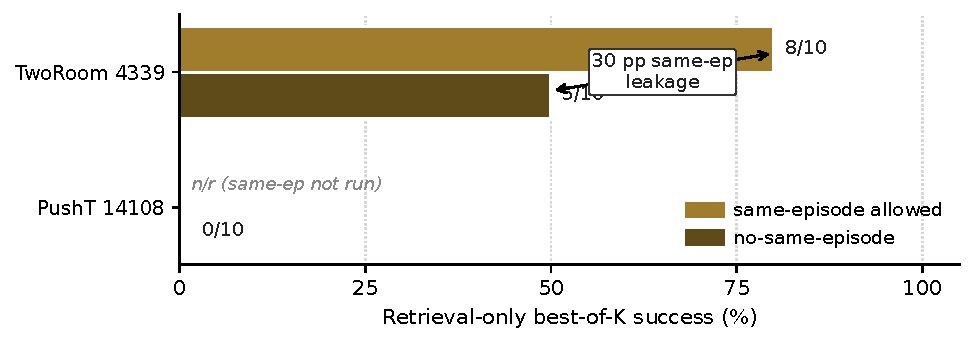
\includegraphics[width=0.92\linewidth]{fig3b_retrieval_leakage.pdf}
  \caption{Retrieval-only leakage diagnostic. Same-episode allowed vs.\ no-same-episode best-of-$K{=}10$ open-loop retrieval on TwoRoom~4339 ($8/10$ vs.\ $5/10$, a $30$-pp leakage delta) and on PushT~14108 (no-same-ep $0/10$; same-ep variant not run, marked n/r).}
  \label{fig:retrieval-leakage}
\end{figure}

\section{TwoRoom 4339 forest plot}
\label{app:tworoom-mechanism-fig}

Figure~\ref{fig:tworoom-mechanism} expands the per-primitive results for the TwoRoom~4339 anchor slice underlying \S\ref{sec:taxonomy}: each row is one primitive cell's success rate at its reported budget, with Wilson $95\%$ binomial confidence intervals as whiskers and $k/n$ labels alongside.

\begin{figure}[ht]
  \centering
  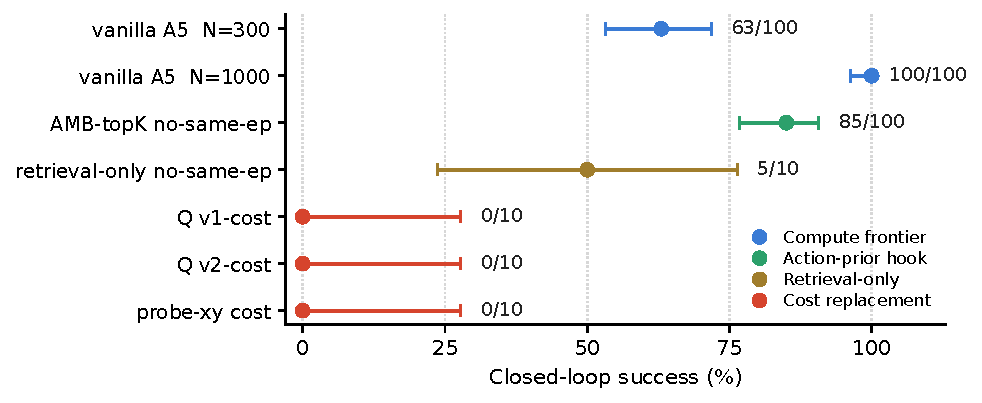
\includegraphics[width=0.92\linewidth]{fig3a_tworoom_mechanism.pdf}
  \caption{TwoRoom~4339 mechanism (forest plot; Wilson 95\% binomial CIs; $k/n$ labels). Vanilla A5 at the published budget $N{=}300$ gives $63/100$, rising to $100/100$ at $N{=}1000$; AMB-topK no-same-ep gives $85/100$ (paired $+22$\,pp over vanilla); retrieval-only no-same-ep gives $5/10$; cost replacements (Q v1/v2, probe-xy) all give $0/10$.}
  \label{fig:tworoom-mechanism}
\end{figure}

\section{Per-slice primitive matrices}
\label{app:slice-matrices}

The compact summary in §\ref{sec:taxonomy} (paragraph after Figure~\ref{fig:taxonomy-showcase}) groups primitives by strand. Tables~\ref{tab:slice-tworoom}--\ref{tab:slice-pusht14108} give the full per-primitive matrix for each anchor slice, preserving exact $k/n$ counts.

\begin{table}[ht]
\centering\small
\caption{TwoRoom 4339 primitive outcomes ($k/n$).}
\label{tab:slice-tworoom}
\begin{tabular}{llr}
\toprule
Primitive & Cell & Outcome \\
\midrule
Default                  & vanilla A5 $N{=}300$        & $63/100$ \\
Compute frontier         & vanilla A5 $N{=}1000$       & $100/100$ \\
Compute frontier (pilot) & vanilla A5 $N{=}3000$       & $3/3$ \\
Action-prior hook        & AMB-topK no-same-ep         & $85/100$ \\
Action-prior hook        & AMB-random same-ep (legacy) & $33/50$ \\
Retrieval-only           & no-same-ep, $K{=}10$         & $5/10$ \\
Retrieval-only           & same-ep allowed, $K{=}10$    & $8/10$ \\
Cost replacement         & Q v1, Q v2, probe-xy         & each $0/10$ \\
Expert replay            & dataset action segment       & success \\
\bottomrule
\end{tabular}
\end{table}

\begin{table}[ht]
\centering\small
\caption{PushT 8314 primitive outcomes ($k/n$).}
\label{tab:slice-pusht8314}
\begin{tabular}{llr}
\toprule
Primitive & Cell & Outcome \\
\midrule
Default            & vanilla A5 $N{=}300$        & $6/20$ \\
Compute frontier   & vanilla A5 $N{=}1000$       & $18/20$ \\
Action-prior hook  & AMB-topK no-same-ep         & $6/20$ \\
Action-prior hook  & AMB-random no-same-ep       & $7/20$ \\
Cost replacement   & contact-cost ($n{=}5$)       & $0/5$ \\
Retrieval-only     & not run                     & n/r \\
Expert replay      & dataset action segment       & success \\
\bottomrule
\end{tabular}
\end{table}

\begin{table}[ht]
\centering\small
\caption{PushT 14108 primitive outcomes ($k/n$).}
\label{tab:slice-pusht14108}
\begin{tabular}{llr}
\toprule
Primitive & Cell & Outcome \\
\midrule
Default                  & vanilla A5 $N{=}300$        & $2/20$ \\
Compute frontier         & vanilla A5 $N{=}1000$       & $2/20$ \\
Compute frontier (pilot) & vanilla A5 $N{=}3000$       & $1/3$ \\
Action-prior hook        & AMB-topK no-same-ep         & $1/20$ \\
Action-prior hook (pilot)& AMB-random no-same-ep        & $0/5$ \\
Cost replacement         & contact-only ($n{=}5$)        & $0/5$ \\
Cost replacement         & probe + penalty ($n{=}5$)     & $0/5$ \\
Retrieval-only           & no-same-ep, $K{=}10$         & $0/10$ \\
Expert replay            & dataset action segment       & success \\
\bottomrule
\end{tabular}
\end{table}

\section{Source-of-record manifest}
\label{app:sources}

Each reported cell maps to one diagnostic JSON. All paths below are under \path{phase1/two_room_planner_ablation/diagnostics/} unless noted; result directories are under \path{phase1/two_room_planner_ablation/results/}. Wilson 95\% CIs are recomputed from \texttt{success\_count}/\texttt{len(results)} in each JSON. The manifest is split into three slice-grouped tables (Tables~\ref{tab:sources-tworoom}--\ref{tab:sources-aggregate}) for readability; paired-difference statistics and the retrieval-quality JSON are in Table~\ref{tab:sources-paired}.

\begin{longtable}{@{}>{\raggedright\arraybackslash}p{2.3cm} >{\raggedright\arraybackslash}p{1.9cm} r >{\raggedright\arraybackslash}p{1.4cm} >{\raggedright\arraybackslash}p{5.4cm}@{}}
\caption{TwoRoom 4339 source-of-record (cells cited in §3 and §4).} \label{tab:sources-tworoom} \\
\toprule
Cell & Cited & $k/n$ & 95\% CI & Diagnostic file \\
\midrule
\endfirsthead
\toprule
Cell & Cited & $k/n$ & 95\% CI & Diagnostic file \\
\midrule
\endhead
\bottomrule
\endfoot
vanilla A5 $N{=}300$ (100 seeds)        & §3.2, Fig~\ref{fig:tworoom-mechanism} & $63/100$  & $[53, 72]$ & \path{tworoom-seed-sweep-ep4339-20260504-142931.json} \\
vanilla A5 $N{=}1000$ (100 seeds)       & §3.2, Fig~\ref{fig:tworoom-mechanism} & $100/100$ & $[96, 100]$ & \path{tworoom-seed-sweep-ep4339-20260504-160559.json} \\
vanilla A5 $N{=}3000$ ($n{=}3$ pilot)    & Tab.~\ref{tab:slice-tworoom}          & $3/3$     & (n=3)       & \path{tworoom-seed-sweep-ep4339-20260503-180739.json} \\
AMB-topK no-same-ep $N{=}300$ (100)     & §4.2, Fig~\ref{fig:tworoom-mechanism} & $85/100$  & $[77, 91]$  & \path{tworoom-bridge-bridge-ep4339-20260504-143425.json} \\
AMB-random same-ep $N{=}300$ (50; legacy) & Tab.~\ref{tab:slice-tworoom}          & $33/50$   & $[52, 78]$  & \path{tworoom-bridge-random-ep4339-20260504-120942.json} \\
Q v1-cost $N{=}300$ ($n{=}10$)            & Tab.~\ref{tab:cost}                  & $0/10$    & $[0, 28]$   & \path{tworoom-q-cost-cumulative-ep4339-20260503-153330.json} \\
Q v2-cost $N{=}300$ ($n{=}10$)            & Tab.~\ref{tab:cost}                  & $0/10$    & $[0, 28]$   & \path{tworoom-q-cost-cumulative-ep4339-20260503-185451.json} \\
probe-xy cost $N{=}300$ ($n{=}10$)        & Tab.~\ref{tab:cost}                  & $0/10$    & $[0, 28]$   & \path{tworoom-probe-cumulative-ep4339-20260503-155032.json} \\
retrieval-only same-ep ($K{=}10$)         & Fig~\ref{fig:retrieval-leakage}      & $8/10$    & $[49, 94]$  & \path{tworoom-retrieval-only-bridge-ep4339-20260503-224837.json} \\
retrieval-only no-same-ep ($K{=}10$)      & Fig~\ref{fig:retrieval-leakage}      & $5/10$    & $[24, 76]$  & \path{tworoom-retrieval-only-bridge-ep4339-20260503-233710.json} \\
\end{longtable}

\begin{longtable}{@{}>{\raggedright\arraybackslash}p{2.3cm} >{\raggedright\arraybackslash}p{1.9cm} r >{\raggedright\arraybackslash}p{1.4cm} >{\raggedright\arraybackslash}p{5.4cm}@{}}
\caption{PushT 8314 / 14108 / 1639 source-of-record.} \label{tab:sources-pusht} \\
\toprule
Cell & Cited & $k/n$ & 95\% CI & Diagnostic file \\
\midrule
\endfirsthead
\toprule
Cell & Cited & $k/n$ & 95\% CI & Diagnostic file \\
\midrule
\endhead
\bottomrule
\endfoot
8314 vanilla A5 $N{=}300$ (20)              & Fig~\ref{fig:pusht-hardcases}    & $6/20$   & $[15, 52]$ & \path{pusht-seed-sweep-ep8314-20260504-180846.json} \\
8314 vanilla A5 $N{=}1000$ (20)             & Fig~\ref{fig:pusht-hardcases}    & $18/20$  & $[70, 97]$ & \path{pusht-seed-sweep-ep8314-20260504-185414.json} \\
8314 AMB-topK no-same-ep (20)               & Fig~\ref{fig:pusht-hardcases}    & $6/20$   & $[15, 52]$ & \path{pusht-bridge-bridge-ep8314-20260504-193759.json} \\
8314 AMB-random no-same-ep (20)             & Fig~\ref{fig:pusht-hardcases}    & $7/20$   & $[18, 57]$ & \path{pusht-bridge-random-ep8314-20260504-230923.json} \\
8314 contact-cost ($n{=}5$)                  & Tab.~\ref{tab:cost}              & $0/5$    & $[0, 43]$  & \path{pusht-contact-contact_plus-ep8314-20260504-082135.json} \\
14108 vanilla A5 $N{=}300$ (20)             & Fig~\ref{fig:pusht-hardcases}    & $2/20$   & $[3, 30]$  & \path{pusht-seed-sweep-ep14108-n300-20260504-200623.json} \\
14108 vanilla A5 $N{=}1000$ (20)            & Fig~\ref{fig:pusht-hardcases}    & $2/20$   & $[3, 30]$  & \path{pusht-seed-sweep-ep14108-n1000-20260504-210645.json} \\
14108 vanilla A5 $N{=}3000$ ($n{=}3$ pilot)  & Tab.~\ref{tab:slice-pusht14108} & $1/3$   & (n=3)       & \path{pusht-seed-sweep-ep14108-20260504-082828.json} \\
14108 AMB-topK no-same-ep (20)              & Fig~\ref{fig:pusht-hardcases}    & $1/20$   & $[1, 24]$  & \path{pusht-bridge-bridge-ep14108-20260504-214619.json} \\
14108 AMB-random no-same-ep ($n{=}5$ pilot)  & Fig~\ref{fig:pusht-hardcases}    & $0/5$    & $[0, 43]$  & \path{pusht-bridge-random-ep14108-20260504-012016.json} \\
14108 retrieval-only no-same-ep ($K{=}10$)   & Fig~\ref{fig:retrieval-leakage}  & $0/10$   & $[0, 28]$  & \path{pusht-retrieval-only-bridge-ep14108-20260504-012600.json} \\
14108 contact-cost (contact-only, $n{=}5$)   & Tab.~\ref{tab:cost}              & $0/5$    & $[0, 43]$  & \path{pusht-contact-contact_only-ep14108-20260504-081432.json} \\
14108 contact-cost (probe+pen, $n{=}5$)      & Tab.~\ref{tab:cost}              & $0/5$    & $[0, 43]$  & \path{pusht-contact-contact_plus-ep14108-20260504-082419.json} \\
1639 AMB-topK no-same-ep ($n{=}5$ regression) & §4 intro                        & $5/5$    & $[57, 100]$ & \path{pusht-bridge-bridge-ep1639-20260504-011843.json} \\
\end{longtable}

\begin{longtable}{@{}>{\raggedright\arraybackslash}p{3.6cm} >{\raggedright\arraybackslash}p{2.4cm} >{\raggedright\arraybackslash}p{2.4cm} >{\raggedright\arraybackslash}p{4.2cm}@{}}
\caption{Aggregate artifacts: four-task grid; Reacher A0 multi-seed Hydra control; Cube hard-case sweep. Per-cell or per-seed JSONs that the aggregate pointer resolves to are listed in the file (or the underlying summary JSON).}
\label{tab:sources-aggregate} \\
\toprule
Artifact & Cited & Coverage & Diagnostic file \\
\midrule
\endfirsthead
\toprule
Artifact & Cited & Coverage & Diagnostic file \\
\midrule
\endhead
\bottomrule
\endfoot
Four-task A0..A5 + $H{=}10$ grid ($\mathit{num\_eval}{=}50$) & §3.1, Tab.~\ref{tab:perturb}, Tab.~\ref{tab:reacher-5seed} & 4 tasks $\times$ 8 cells & \path{grid-path2-summary.json} \\
Reacher A0 5-seed Hydra control                              & Appx.~\ref{app:reacher}                                       & 5 seeds; 44/42/42/46/38 & \path{reacher-multiseed-a0.json} \\
Cube hard-case sweep (3 episodes $\times$ 4 cells $\times$ 5 paired seeds) & Tab.~\ref{tab:cube-hardcase}                & $0/60$ pooled            & \path{cube-hardcase-sweep-summary.json} \\
\end{longtable}

\begin{longtable}{@{}>{\raggedright\arraybackslash}p{5.4cm} >{\raggedright\arraybackslash}p{2.6cm} >{\raggedright\arraybackslash}p{4.4cm}@{}}
\caption{Paired-difference / McNemar JSONs and retrieval-quality JSON.}
\label{tab:sources-paired} \\
\toprule
Comparison set & Cited & Diagnostic file \\
\midrule
\endfirsthead
\toprule
Comparison set & Cited & Diagnostic file \\
\midrule
\endhead
\bottomrule
\endfoot
TwoRoom 4339 paired CIs + McNemar (AMB-topK / $N{=}1000$ / $N{=}300$) & Tab.~\ref{tab:paired-stats} & \path{tworoom-paired-ci-ep4339.json} \\
PushT 8314 / 14108 paired CIs + McNemar                                & Tab.~\ref{tab:paired-stats} & \path{pusht-paired-ci-stabilizer.json} \\
TwoRoom 4339 top-$K$ vs random decoded endpoint distances              & Appx.~\ref{app:retrieval-quality}, Tab.~\ref{tab:retrieval-quality} & \path{tworoom-amb-retrieval-quality-ep4339-20260504-103518.json} \\
\end{longtable}

\section{Compute resources}
\label{app:compute}

Per-seed wall-clock for the headline cells: TwoRoom A5 $N{=}300$ approximately $120$ s/seed; A5 $N{=}1000$ approximately $390$ s/seed; AMB-topK $N{=}300$ approximately $180$ s/seed (including offline-chunk-database build at experiment startup). Push-T cells: A5 $N{=}300$ approximately $55$ s/seed; A5 $N{=}1000$ approximately $130$ s/seed; AMB-topK $N{=}300$ approximately $80$ s/seed. The complete protocol on Two-Room~$4339$ and the two Push-T hard episodes (compute frontier + cost replacement + leakage + AMB variants + paired-difference statistics) ran on a single GPU host with thread limits enforced (\texttt{OMP\_NUM\_THREADS}=$4$, etc.). Hardware-accelerator type and memory are not fully recorded for every run; we report total wall-clock per cell where available rather than total energy.

\input{checklist}

\end{document}
